% Version 0; preprint format; Outline of paper II by Song Huang
% Version 1; preprint format; Edited by Jenny Greene
% Version 2; preprint format; Edited by Song Huang
% Version 3; preprint format; Edited by Alexie Leauthaud
% Version 4; preprint format; Edited by Song Huang
% Version 5; preprint format; Edited by Jenny Greene and Song Huang


\documentclass[a4paper,fleqn,usenatbib]{mnras}

% Packages
\usepackage{deluxetable}
\usepackage{newtxtext,newtxmath}
\usepackage[T1]{fontenc}
\usepackage{ae,aecompl}
\usepackage{amssymb, amsmath}
\usepackage{graphicx}
\usepackage{natbib}
\usepackage{url}
\usepackage{hyperref}
\usepackage{float}
\usepackage[usenames, dvipsnames]{color}

% Package Settings
\hypersetup{colorlinks=true,
            citecolor=cyan,
            linkcolor=cyan,
            filecolor=magenta,      
            urlcolor=cyan}
\urlstyle{same}

% Figure extention
\DeclareGraphicsExtensions{.pdf,.png,.jpg}

%%%%%%%%%%%%: User Defined Commands %%%%%%%%%%%%

% Song Huang's definition 
\def\arcsec{{\prime\prime}}
\def\arcmin{{\prime}}
\def\degree{{\circ}}
\def\h{\hskip -3 mm}
\def\aa{{A\&A}}
\def\aas{{ A\&AS}}
\def\aj{{AJ}}
\def\al{$\alpha$}
\def\bet{$\beta$}
\def\amin{$^\prime$}
\def\annrev{{ARA\&A}}
\def\apj{{ApJ}}
\def\apjs{{ApJS}}
\def\asec{$^{\prime\prime}$}
\def\deg{$^{\circ}$}
\def\ddeg{{\rlap.}$^{\circ}$}
\def\dsec{{\rlap.}$^{\prime\prime}$}
\def\cc{cm$^{-3}$}
\def\flamb{erg s$^{-1}$ cm$^{-2}$ \AA$^{-1}$}
\def\flux{erg s$^{-1}$ cm$^{-2}$}
\def\fnu{erg s$^{-1}$ cm$^{-2}$ Hz$^{-1}$}
\def\hst{{\textit{HST}}}
\def\kms{km s$^{-1}$}
\def\lamb{$\lambda$}
\def\lax{{$\mathrel{\hbox{\rlap{\hbox{\lower4pt\hbox{${\sim}$}}}\hbox{$<$}}}$}}
\def\gax{{$\mathrel{\hbox{\rlap{\hbox{\lower4pt\hbox{${\sim}$}}}\hbox{$>$}}}$}}
\def\simlt{\lower.5ex\hbox{$\; \buildrel < \over {\sim} \;$}}
\def\simgt{\lower.5ex\hbox{$\; \buildrel > \over {\sim} \;$}}
\def\micron{{$\mu$m}}
\def\mnras{{MNRAS}}
\def\nat{{Nature}}
\def\pasp{{PASP}}
\def\perang{\AA$^{-1}$}
\def\peryr{yr$^{-1}$}
\def\reference{\noindent\pp}
\def\refindent{\par\noindent\parskip=2pt\hangindent=3pc\hangafter=1 }
\def\sb{mag~arcsec$^{-2}$}
\def\lsun{$L_\odot$} 
\def\msun{$M_\odot$}
\def\sigs{$\sigma_*$}
\newcommand{\lt}{<}
\newcommand{\gt}{>}

\def\etal{{\ et al.~}}
\def\galfit{{\tt GALFIT}}
\def\ser{{S\'{e}rsic\ }}
\def\redm{\texttt{redMaPPer}}
\def\cmodel{\texttt{cModel}}
% Samples
\def\rbcg{\texttt{cenHighMh}}
\def\nbcg{\texttt{cenLowMh}}
\def\redbcg{{$\lambda \ge 30$}}
\def\nonbcg{{$\lambda < 20$}}
% Mass related 
\def\mstar{{$M_{\star}$}}
\def\mhalo{{$M_{\mathrm{200b}}$}}
\def\logms{{$\log (M_{\star}/M_{\odot})$}}
\def\logmh{{$\log (M_{\mathrm{200b}}/M_{\odot})$}}
\def\logmhalo{{$\log (M_{\mathrm{200b}}/M_{\odot})$}}

\def\minn{{$M_{\star,10\mathrm{kpc}}$}}
\def\meff{{$M_{\star,15\mathrm{kpc}}$}} 
\def\mtot{{$M_{\star,100\mathrm{kpc}}$}}
\def\mout{{$M_{\star,150\mathrm{kpc}}$}}
\def\mmax{{$M_{\star,\mathrm{Max}}$}}
\def\mgama{{$M_{\star,\mathrm{GAMA}}$}}
\def\mcmodel{{$M_{\star,\mathrm{cModel}}$}}

\def\logminn{{$\log (M_{\star,10\mathrm{kpc}}/M_{\odot})$}}
\def\logmtot{{$\log (M_{\star,100\mathrm{kpc}}/M_{\odot})$}}
\def\logmout{{$\log (M_{\star,150\mathrm{kpc}}/M_{\odot})$}}
\def\logmmax{{$\log (M_{\star,\mathrm{Max}}/M_{\odot})$}}
\def\logmgama{{$\log (M_{\star,\mathrm{GAMA}}/M_{\odot})$}}
\def\logmcmodel{{$\log (M_{\star,\mathrm{cModel}}/M_{\odot})$}}

\def\m2l{{$M_{\star}/L_{\star}$}}
\def\s2n{{$\mathrm{S}/\mathrm{N}$}}
\def\mden{{$\mu_{\star}$}}

\def\insitu{{\textit{in situ}}}
\def\exsitu{{\textit{ex situ}}}

% Commenting:
\newcommand{\xxx}[1]{\textcolor{red}{\textbf{XXX}}}
\newcommand{\todo}[1]{\textcolor{red}{\textbf{TODO:~#1}}}
\newcommand{\plan}[1]{\textcolor{cyan}{#1}}
\newcommand{\addref}{{\textcolor{red}{REF}}}
\newcommand{\note}[2]{\textcolor{blue}{\textbf{[Comment (#1): #2]}}}
\newcommand{\song}[1]{\textcolor{magenta}{\textbf{[Song: #1]}}}
\newcommand{\alexie}[1]{\textcolor{blue}{\textbf{[Alexie: #1]}}}
\newcommand{\jenny}[1]{\textcolor{Bittersweet}{\textbf{[Jenny: #1]}}}
\newcommand{\kevin}[1]{\textcolor{green}{\textbf{[Kevin: #1]}}}
\newcommand{\update}[1]{\textcolor{PineGreen}{#1}}

%% ------------------------------------------------------------------------------------ %% 
%% Title and Affiliations 
%% ------------------------------------------------------------------------------------ %% 

%\title[Structure and Environment of Massive Galaxies]{
%       A Detection of the Environmental Dependence of the Stelllar and haloes
%       of Massive Central Galaxies}

\title[Structure and Environment of Massive Galaxies]{
       A Detection of the Environmental Dependence of the Sizes and Stellar Haloes
       of Massive Central Galaxies}
       
\author[S. Huang et al.]{
        Song Huang$^{1,2}$\thanks{E-mail: song.huang@ipmu.jp (SH)},
        Alexie Leauthaud$^{1}$,
        Jenny Greene$^{4}$,
        Kevin Bundy$^{3}$,
        \newauthor
        Yen-Ting Lin$^{5}$,
        Masayuki Tanaka$^{6}$,
        Rachel Mandelbaum$^{7}$,
        Satoshi Miyazaki$^{5,8}$,
        \newauthor
        Yutaka Komiyama$^{5,8}$
        \\
        $^{1}$Department of Astronomy and Astrophysics, University of California 
              Santa Cruz, 1156 High St., Santa Cruz, CA 95064, U.S.A\\
        $^{2}$Kavli-IPMU, The University of Tokyo Institutes for Advanced Study, 
              the University of Tokyo (Kavli IPMU, WPI), Kashiwa 277--8583, Japan\\              
        $^{3}$UCO/Lick Observatory, University of California, Santa Cruz,
              1156 High Street, Santa Cruz, CA 95064, USA\\
        $^{4}$Department of Astrophysical Sciences, Peyton Hall,
              Princeton University, Princeton, NJ 08540, USA \\
        $^{5}$National Astronomical Observatory of Japan, 2--21--1 Osawa, Mitaka, 
              Tokyo 181--8588, Japan\\
        $^{6}$Academia Sinica Institute of Astronomy and Astrophysics, 
              P.O. Box 23--141, Taipei 10617, Taiwan\\
        $^{7}$McWilliams Center for Cosmology, Department of Physics, 
              Carnegie Mellon University, Pittsburgh, PA 15213, USA\\
        $^{8}$SOKENDAI (The Graduate University for Advanced Studies), Mitaka,
              Tokyo, 181--8588, Japan
        }   
%% ------------------------------------------------------------------------------------ %% 
\date{Accepted XXX. Received YYY; in original form ZZZ}        
\pubyear{2017}                                  
  
%% ------------------------------------------------------------------------------------ %% 
%% Header and Version 
%% ------------------------------------------------------------------------------------ %% 

\begin{document}

\label{firstpage}
\pagerange{\pageref{firstpage}--\pageref{lastpage}}

\maketitle

%% ------------------------------------------------------------------------------------ %% 
%% Abstract and Keywords 
%% ------------------------------------------------------------------------------------ %% 

\begin{abstract}  

    We use ${\sim}100$ deg$^2$ of deep ($>28.5$ \sb{} in $i$-band), high-quality 
    (median 0.6\asec seeing) imaging data from the Hyper Suprime--Cam (HSC) survey 
    to investigate the halo mass dependence of the surface mass density profiles 
    and outer stellar envelopes of massive galaxies. 
    The $i$-band images from HSC survey reach ${\sim}4$ magnitudes deeper than SDSS 
    and enable us to directly trace stellar mass distributions to 100 kpc without 
    requiring stacking.  
    We conclusively show that at fixed stellar mass, the stellar profiles of massive 
    galaxies depend on the masses of their dark matter halos. 
    On average, massive central galaxies with \logmtot{}$>11.6$ in more massive halos 
    at $0.3 < z < 0.5$ have shallower inner stellar mass density profiles 
    (within ${\sim}10$-$20$ kpc) and more prominent outer envelopes. 
    These differences translate into a halo mass dependence of the 
    mass--size relation: central galaxies in halos with \logmh{}$>14.0$ are 
    $\sim 20$\% larger in $R_{\mathrm{50}}$ at fixed \mtot{}.  
    Such dependence is also reflected in the relationship between the stellar mass 
    within 10 and 100 kpc. 
    Comparing to the mass--size relation, the \mtot{}--\minn{} relation avoids the 
    ambiguity in the definition of size, and can be straightforwardly compared with 
    simulations. 
    Our results demonstrate that, with deep images from HSC, we can quantify the 
    connection between halo mass and the outer stellar halo, which may provide new 
    constraints on the formation and assembly of massive central galaxies.
    
\end{abstract}

\begin{keywords}
    galaxies: elliptical and lenticular, cD --
    galaxies: formation --
    galaxies: photometry -- 
    galaxies: structure -- 
    galaxies: haloes
\end{keywords}


%% ------------------------------------------------------------------------------------ %% 
%% Main Text
%% ------------------------------------------------------------------------------------ %% 


%% ------------------------------------------------------------------------------------ %% 
%% Introduction 
%% ------------------------------------------------------------------------------------ %% 

\section{Introduction}
    \label{sec:intro}
    
    A key discovery in the last 
    decade has been the dramatic structural transformation of massive quiescent 
    galaxies \citep[e.g.][]{Trujillo2006, vanDokkum2008, Cimatti2008, Damjanov2009, 
    vanderWel2011, Szomoru2012, Patel2013} from $z \approx 2$ to the present day. 
    These observations suggest that the progenitors of $z{\sim} 0$ massive early-type 
    galaxies (ETGs) need to increase their effective radii ($R_{\rm e}$) by a factor 
    of 2--4 over a time span of 10 Gyrs (e.g. \citealt{Newman2012, vdWel2014}). 
    This observational result spurred the development of the ``two-phase'' formation
    scenario for massive ETGs (e.g. \citealt{Oser2010, Oser2012}),
    in which galaxies form a compact central region at $z\sim 2$ through highly 
    dissipative processes (e.g. gas-rich mergers or cold gas-accretion;
    \citealt{Hopkins2008, Dekel2009}). 
    They subsequently assemble extended stellar haloes via dry mergers 
    \citep[e.g,][]{Naab2006, Khochfar2006, Oser2010, Oser2012} which can cause 
    significant size growth at late times. 
    An alternative explanation for size growth, progenitor bias, hypothesizes that 
    larger ETGs were quenched more recently, but this explanation is still under 
    active debate (e.g. \citealt{Newman2012, Carollo2013, Poggianti2013, Belli2015,
    Keating2015, Fagioli2016}). 
    
    There have been multiple observational attempts to test the two-phase 
    formation scenario using galaxies at low redshift, by investigating surface 
    brightness or mass density profiles (e.g. \citealt{Huang2013a, Huang2013b, 
    Oh2017}, optical color gradients (e.g. \citealt{LaBarbera2010, LaBarbera2012}), 
    and stellar population gradients \citep[e.g.,][]{Coccato2010, Coccato2011, 
    Greene2015, Barbosa2016}. 
    Although these observations are generally consistent with the two-phase scenario, 
    this picture still faces a key puzzle: whether or not sizes and profiles of galaxies 
    depend on the mass of their host dark matter halos.
 
    According to the two-phase formation scenario, the late time growth of massive 
    ETGs is intrinsically tied to the growth of their host dark matter haloes 
    (e.g. \citealt{Leauthaud2012, Behroozi2013, Shankar2013}). 
    Massive ETGs living at the centers of more massive haloes should be subject to 
    higher merger rates compared to ETGs with similar stellar mass but living in less 
    massive dark matter haloes. 
    A natural prediction of this picture is therefore that the structures of 
    massive ETGs should depend on their ``environment''\footnote{There are 
    multiple definitions of ``environment'' in the literature.  
    In this work, we use ``environment'' and halo mass interchangeably.}.
    Theoretical models based on the two-phase formation scenario predict an 
    environmental dependence of the stellar mass--effective radius relation for 
    ETGs (\mstar{}--$R_{\rm e}$; 
    e.g., \citealt{Shen2003, Guo2009}): the sizes of massive ETGs in more massive 
    haloes should be larger than those in less massive haloes at fixed \mstar{} 
    (e.g. \citealt{Shankar2013, Shankar2014}). 
    Yet, solid evidence of this effect at low redshift is still missing 
    (e.g. \citealt{Nair2010, HCompany13}; but also see \citealt{Yoon2017}).
    
    %However, while hints of an environmental dependence in the mass-size relation have 
    %been spotted at high-$z$ (e.g. \citealt{Papovich2012, Lani2013, Delaye2014}; but 
    %also see \citealt{Rettura2010}). 
    
	% Song: Actually the Illustris paper suggests that, for massive galaxies, 
	%       even the inner region is dominated by accreted stars. 
	
    Testing this prediction requires deep imaging of ETGs in order to probe the 
    accreted component (the stellar halo) which can extend to 100 kpc and 
    beyond \citep[eg.,][]{hscMassiveI}. 
    This is observationally challenging as the surface brightness profiles of massive 
    ETGs decline rapidly with typical values of $\mu > 26.0$ \sb{} in $i$-band at 100 
    kpc and at $z\sim0.3$. 
    In \citet[][Paper I hereafter]{hscMassiveI}, we showed that deep, 
    multi-band imaging from the Subaru Strategic Program (SSP; \citealt{HSC-SSP,
    HSC-DR1}) using Hyper Suprime-Cam (HSC; \citealt{Miyazaki2012}, 
    Miyazaki in~prep.) allows us to extract robust surface stellar
    mass density (\mden{}) profiles for {\it individual} galaxies with 
    \logms{}$>11.4$ at $0.3 < z < 0.5$ and out to 100 kpc. 
    In Paper I, we characterized the stellar mass profiles of massive ETGs, and 
    showed that there is a large intrinsic scatter in the \mden{} stellar halos of
    massive galaxies on 100 kpc scales. 
    In this paper, we now investigate whether or not the large scatter in the outer 
    profiles of massive galaxies correlate with halo mass. 
    We conclusively show that the sizes and stellar halos of massive central galaxies 
    depend on dark matter halo mass. 
    In other terms, we reveal the halo mass dependence of the mass-size relation 
    for massive ETGs.   
    
%    with the help of HSC images of a large sample 
%    of massive ETGs and the \redm{} cluster catalog (e.g.\ \citealt{Rykoff2014}; 
%    \citealt{Rozo2015b}; please see \S \ref{sec:data} for details)
    
    This paper is organized as follows. 
    In \S \ref{sec:data} we briefly introduce the sample selection and the data 
    reduction processes.  
    Please refer to \citet{hscMassiveI} for more technical details.
    Our main results are presented in \S \ref{sec:result} and discussed in 
    \S \ref{sec:discussion}. 
    Section \S \ref{sec:summary} presents our summary and conclusions.

    Magnitudes use the AB system (\citealt{Oke1983}), and are corrected for Galactic 
    extinction using calibrations from \citet{Schlafly11}. 
    We assume $H_0$ = 70~km~s$^{-1}$ Mpc$^{-1}$, ${\Omega}_{\rm m}=0.3$, 
    and ${\Omega}_{\rm \Lambda}=0.7$.
    Stellar mass is denoted \mstar{} and has been derived using a Chabrier Initial Mass 
    Function (IMF; \citealt{Chabrier2003}). Halo mass is defined as 
    $M_{\rm 200b}\equiv M(<r_{\rm 200b})=200\bar{\rho} 
    \frac{4}{3}\pi r_{\rm 200b}^3$ where $r_{\rm 200b}$
    is the radius at which the mean interior density is equal to 200 times
    the mean matter density ($\bar{\rho}$). 
    As in \citet{hscMassiveI}, we do not attempt to decompose or distinguish any  
    potential ``intra-cluster'' 
    component (ICL; e.g. \citealt{Carlberg1997, Lin2004, Gonzalez2005, Mihos2005}). 
    
%% ------------------------------------------------------------------------------------ %% 

%% ------------------------------------------------------------------------------------ %% 
  \begin{figure*}
      \centering 
      \includegraphics[width=\textwidth]{fig/redbcg_m100_m10_compare}
      \caption{
          Three-color images for a subsample of massive galaxies at $z{\sim}0.4$. 
          All of these massive galaxies have very similar \mstar{} within a 10 kpc 
          elliptical aperture 
          ($11.2<\log (M_{\star,10\ \mathrm{kpc}}/M_{\odot})<11.3$). 
          The dash-line circle at the top-left figure indicates $R=$10 kpc.
          These galaxies are rank-ordered from top to bottom and from left to right 
          by their \mstar{} within a 100 kpc elliptical aperture which varies 
          from $10^{11.2} M_{\odot}$ to $10^{11.7} M_{\odot}$. 
          At fixed ``inner'' mass (\minn{}), massive galaxies display significant
          diversity in their outer profiles. 
          Red boxes indicate galaxies from dark matter haloes that are more massive 
          than ${\sim} 10^{14.0} M_{\odot}$. 
          }
      \label{fig:m100_m10_color}
  \end{figure*}
%% ------------------------------------------------------------------------------------ %% 

%% ------------------------------------------------------------------------------------ %% 
  \begin{figure*}
      \centering 
      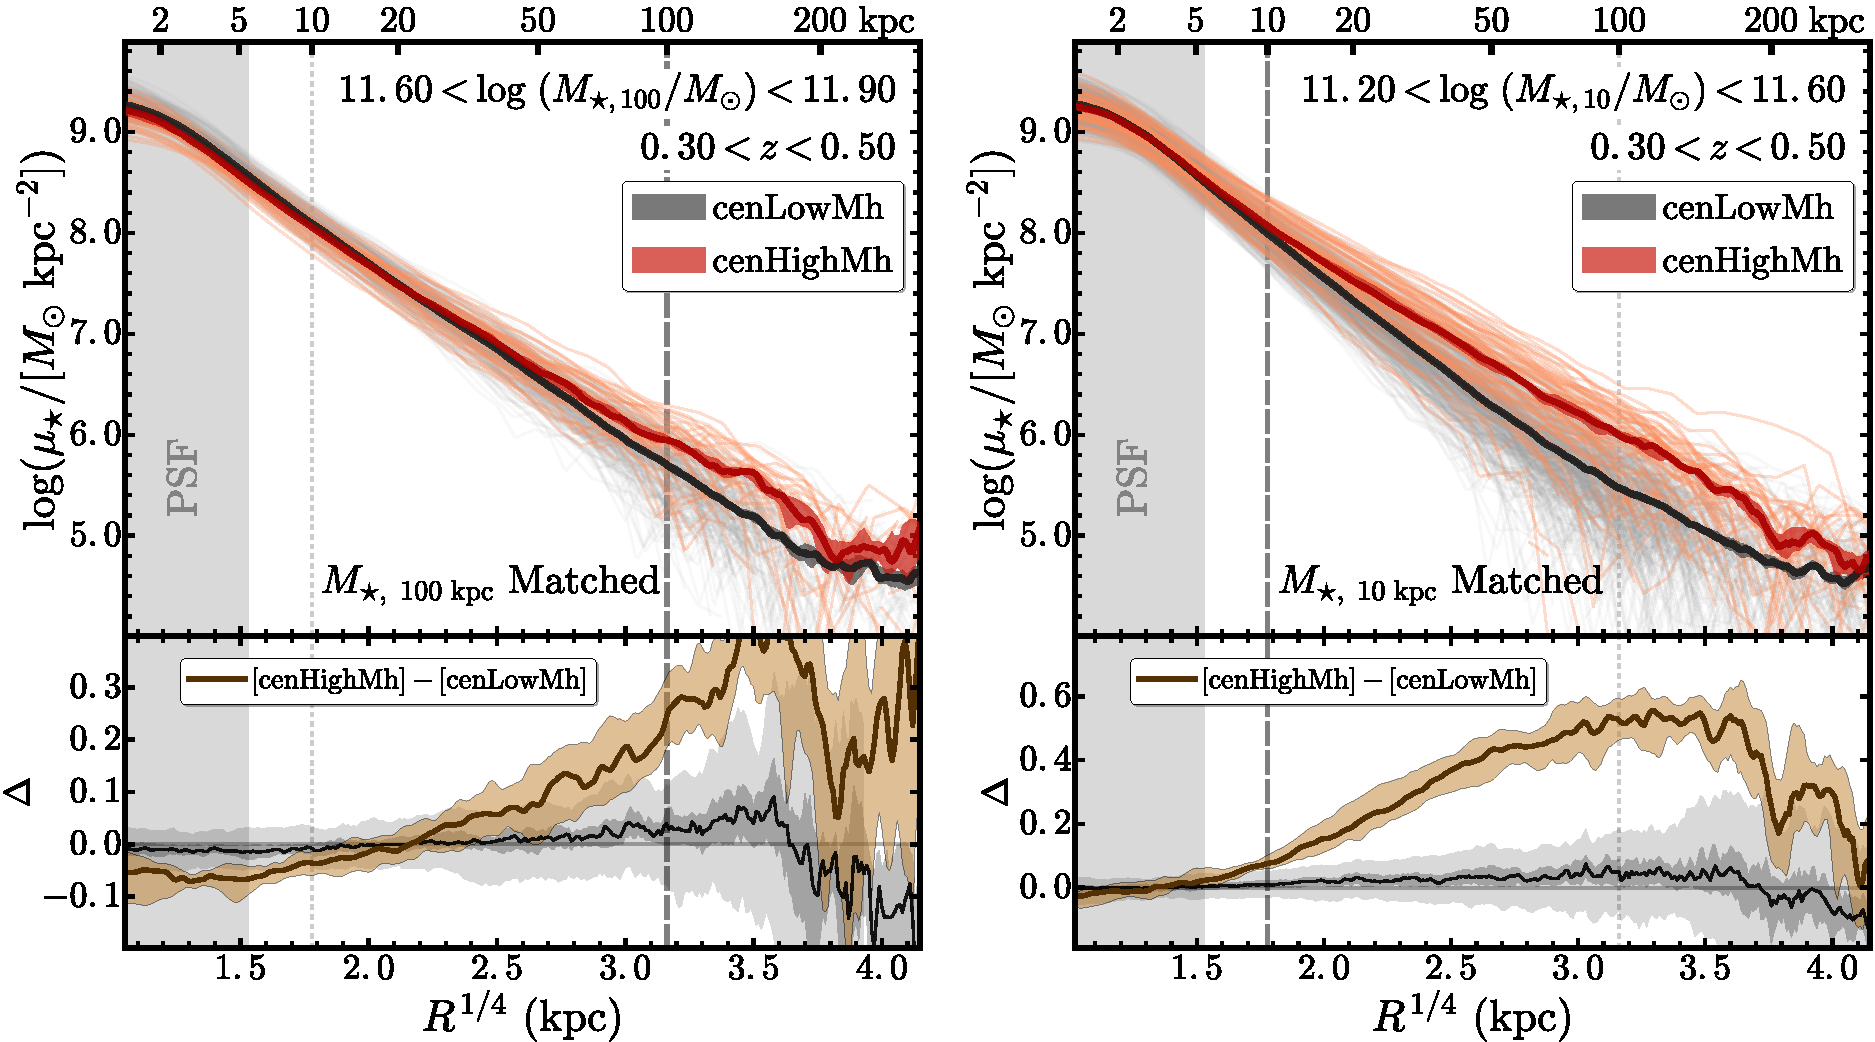
\includegraphics[width=\textwidth]{fig/redbcg_prof_1}
      \caption{
          The environmental dependence of the stellar mass profiles of massive central 
          galaxies. 
          Left: halo mass dependence of galaxy profiles at fixed ``total'' stellar mass 
          (\mtot{}). 
          Right: halo mass dependence of galaxy profiles at fixed ``inner-mass'' 
          (\minn{}). Orange and red lines correspond to central galaxies living in 
          haloes with \logmh{} $\geq 14.2$. 
          Black and grey lines correspond to central galaxies living in haloes with 
          \logmh{} $\leq 14.0$. 
          Thin lines show the profiles of individual galaxies while thick lines show 
          the median profile. 
          The uncertainty on the median profile is given by the shaded region and is 
          computed via bootstrap resampling. 
          Brown lines in the bottom panels show the relative difference between  
          two median profiles 
          ($\Delta = \log(\mu_{\star, \mathrm{cenHighMh}}) - 
          \log(\mu_{\star, \mathrm{cenLowMh}}$). 
          Errors on the difference between the two profiles are also computed 
          via bootstrap.
          The grey shaded regions show a Monte Carlo test to asses how likely is it to 
          obtain $\Delta$ from random sub-samples of the data. 
          To compute the grey shaded regions, we first mix the two samples 
          (\rbcg{} and \nbcg{}), then draw sub-samples of galaxies from the mixed 
          population and compute $\Delta$ in the same fashion as for our fiducial 
          signal. 
          We repeat this process 5000 times.  
          The dark-grey shaded region (light-grey shaded region) shows the 1-$\sigma$ 
          (3-$\sigma$) fluctuations in $\Delta$ from these 5000 draws.
          }
      \label{fig:prof_1} 
  \end{figure*}
%% ------------------------------------------------------------------------------------ %% 

%% ------------------------------------------------------------------------------------ %% 
  \begin{figure*}
      \centering 
      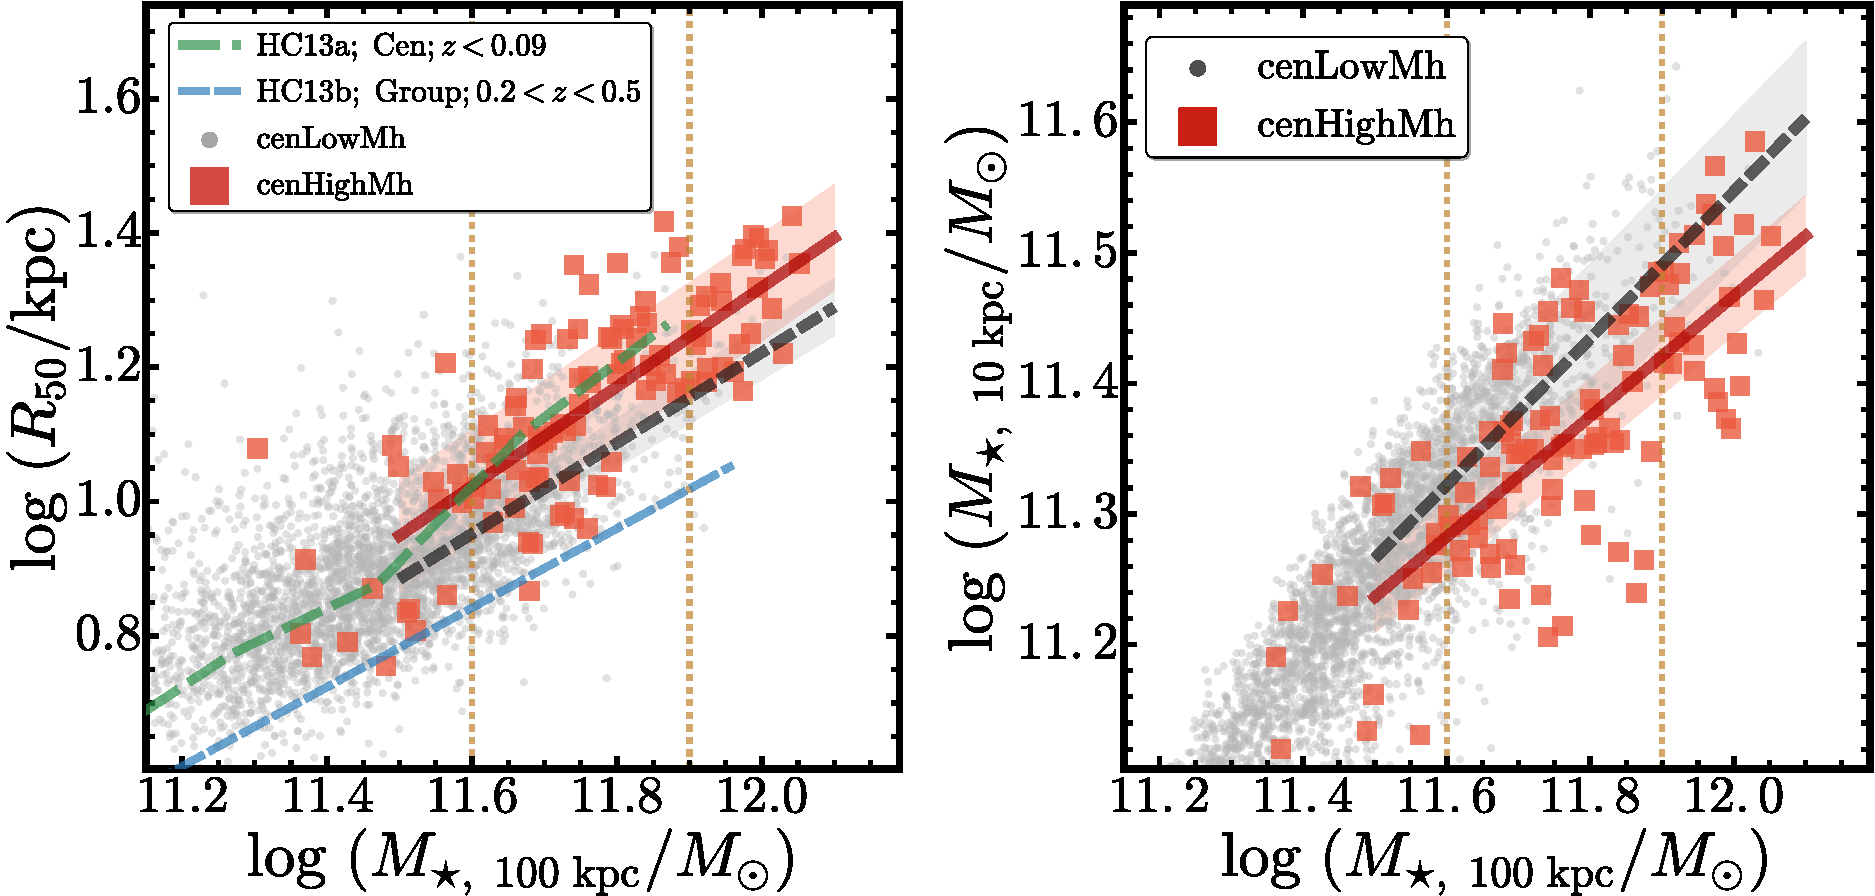
\includegraphics[width=\textwidth]{fig/redbcg_scaling_relation}
      \caption{
          \textbf{Left}: The mass-size relations for \rbcg{} (orange squares) and 
          \nbcg{} (grey dots) galaxies. 
          Two vertical lines highlight our $11.6<$ \logms{} $<11.9$ mass bin. 
          The red solid line shows the best fit mass-size relation for \rbcg{} and the 
          grey dashed line shows the best fit relation for \nbcg{}. 
          Shaded regions in lighter colors show the 1-$\sigma$ uncertainties
          from MCMC sampling.  
          The green dashed line shows the mass-size relation for nearby central 
          galaxies in massive groups from \citet{HCompany13}. 
          \textbf{Right:} The relations between \mtot{} and \minn{} for the 
          \rbcg{} and \nbcg{} galaxies, along with the best-fit scaling relations for 
          both samples.
          }
      \label{fig:scaling_relation} 
  \end{figure*}
%% ------------------------------------------------------------------------------------ %% 

%% ------------------------------------------------------------------------------------ %% 
%% Sample Selection and Data Reduction
%% ------------------------------------------------------------------------------------ %% 
\section{Sample Selection and Data Reduction}
    \label{sec:data}
    
    We refer the reader to Paper I for an in-depth description of the sample selection 
    and data reduction processes. 
    Here, we briefly summarize the main steps.
    
    We use imaging data from the HSC internal data release 
    \texttt{S15B}, which is very similar to the Public Data Release 1 
    (\citealt{HSC-DR1} and covers ${\sim} 110$ deg$^2$ in all five-band ($grizy$) to 
    the full depth in the Wide field. 
    The data are reduced by \texttt{hscPipe 4.0.2}, a derivative of the 
    Large Synoptic Survey Telescope (LSST) pipeline (e.g.\ \citealt{Juric2015}; 
    \citealt{Axelrod2010}), modified for HSC (\citealt{HSC-PIPE}).
    The pixel scale of the reduced image is $0.168$\asec{}.
    We use $i$-band images for extracting surface brightness profiles. 
    HSC $i$-band images are typically 3--4 mag deeper than SDSS 
    (Sloan Digital Sky Survey; e.g. \citealt{SDSS-DR7, SDSS-DR8, SDSS-DR12})  
    and have superb seeing conditions (mean $i$-band seeing has FWHM$=0.6$\asec{}).
    
    In Paper~I, we select a sample of 25286 bright galaxies with spectroscopic 
    redshifts or reliable ``red-sequence'' photometric redshifts (\citealt{Rykoff2014}) 
    at $0.3<z<0.5$. 
    Within this redshift range, we have a large enough volume 
    ($\sim5\times 10^6$ Mpc$^3$) to sample the galaxy stellar mass function above 
    \logms$>11.6$, we can spatially resolve galaxies profiles to $\sim 5$ kpc 
    ($1.0^{\arcsec}$ corresponds to 4.4 and 6.1 kpc at $z=0.3$ and 0.5), and we can 
    safely ignore structural evolution over our redshift range ($\sim$1.5 Gyr of 
    time span).
    
    We derive $i$-band surface brightness profiles out to 100 kpc after carefully 
    masking out surrounding neighbors and accounting for the subtraction of the 
    background light. 
    We use the broadband spectral energy distributions (SED) fitting code 
    \texttt{iSEDFit}\footnote{http://www.sos.siena.edu/~jmoustakas/isedfit/} 
    (\citealt{Moustakas13}) to measure \m2l{} ratios and $k$--corrections using 
    five-band forced \cmodel{} magnitudes from \texttt{hscPipe}. 
    We assume a \citet{Chabrier2003} IMF, the Flexible Stellar Population 
    Synthesis models\footnote{http://scholar.harvard.edu/cconroy/sps-models}
    (FSPS; \texttt{v2.4}; \citealt{FSPS}, \citealt{Conroy2010}), the 
    \citet{Calzetti2000} extinction law, and a simple delayed-$\tau$ model for 
    star formation histories (SFH). 
    Using HSC data, we can measure the \mden{} profiles of massive galaxies to 
    $\sim 100$ kpc and we integrate these profiles within elliptical isophotal
    apertures at different physical radii. 
    As explained in Paper~I, here we focus on the two following metric masses:
        
    \begin{itemize}
    
        \item stellar mass within 10 kpc (hereafter noted \minn{}) which we use 
            as a proxy for the stellar mass of the \textit{in situ} stellar 
            component. 
            This is motivated both by recent observations and simulations 
            (e.g.~\citealt{vanDokkum2010}, \citealt{RodriguezGomez2016}). 
            The value of 10 kpc that we quote here corresponds to the radius of the 
            major axis of the isophotal ellipse.
            
        \item stellar mass within 100 kpc (hereafter noted \mtot{}). 
            We use \mtot{} as a proxy of the ``total'' stellar mass. 
            In Paper~I we showed that \mtot{} recovers more light compared to 
            HSC \cmodel{} photometry with offsets that can be a large as 0.2 dex 
            in magnitude.        
               
   \end{itemize}
   
   We use these two simple metric masses to explore the \mstar{}-dependence of the 
   fraction of accreted stars, and reveal the diversity of stellar envelopes among 
   massive galaxies. 
   In practice, we also have the full profiles for each galaxy and can cast our 
   results in terms of the full stellar mass profiles. 
   However, in many cases we find it more useful to display figures using the more 
   simple \minn{} and \mtot{} quantities. 
   In Figure \ref{fig:m100_m10_color}, we highlight the diversity of galaxies as a 
   function of \minn{} and \mtot{}. 
   Figure \ref{fig:m100_m10_color} shows a random subsample of massive galaxies with 
   very similar \minn{} that have large range of \mtot{}. 
   We will use these two apertures masses to guide our comparisons of massive galaxies 
   as a function of environment.  
    
%% ------------------------------------------------------------------------------------ %%    
\subsection{Massive Central Galaxies from Different Environments}
    \label{ssec:cen}
         
    In this work, we focus on massive galaxies with \mtot{} $>10^{11.6}$~\msun{}. 
    In Paper~I, we demonstrate that this sample is almost mass complete over our full 
    redshift range. 
    In addition to the mass cut above, we also limit our sample to galaxies that live 
    at the centers of their own dark matter haloes-- so-called ``central'' galaxies. 
    We use the \redm{} \texttt{v5.10} \citep{Rykoff2014, Rozo2015b} cluster catalog 
    to help us construct a central galaxy sample.
    
    %Central galaxies are important to the study of galaxy-halo connection and follow 
    %stellar mass--halo mass relation (SHMR; e.g. \citealt{Leauthaud2012, 
    %Behroozi2013, Kravtsov2014, Tinker2017}) at high-\mstar{}.
 
    Firstly, we select 68 massive central galaxies from \redm{} clusters 
    with richness ($\lambda$) $\geq 30$, and the probability of true central galaxy 
    ($P_{\mathrm{Cen}}$) $\geq 0.7$, and \logmtot{}$>11.5$ 
    at $0.3 < z < 0.5$ (63/68 have \logmtot{}$>11.6$). 
    This $\lambda$ limit is chosen to mitigate incompleteness in the cluster catalog
    at the high end of our redshift window. 
    The $P_{\mathrm{Cen}}$ limit is selected to exclude low probability candidate of 
    central galaxy. 
    Based on the \mhalo{}-$\lambda$ relation calibrated by \citet{Simet2016}, these 
    correspond to central galaxies living in halos with \mhalo{}$>10^{14.2}$~\msun{}. 
    This calibration is consistent with other works (e.g. \citealt{Saro2015, Farahi2016, 
    Melchior2016, Murata2017}). 
    The median richness of the sample is $\lambda \approx 41$ 
    (\mhalo{}$\approx 2.2 \times 10^{14}$~\msun{}), and there are 
    only 44 central galaxies in clusters with $\lambda>50$ 
    (\mhalo{}$\approx 3.0 \times 10^{14}$~\msun{}).
    We will refer to this sample of \textbf{central galaxies in massive haloes} as 
    the \rbcg{} sample.
    
    Secondly, we build a complementary sample of central galaxies in lower-mass haloes
    by excluding all galaxies that are in any \redm{} cluster with $\lambda > 20$.
    We convert their $\lambda$ into $M_{\mathrm{200b}}$ using calibration by 
    \citet{Simet2016}. 
    Then we estimate the $R_{\mathrm{200b}}$ of each cluster using the method in 
    \citet{Diemer2015}. 
    We further exclude all galaxies within a cylinder around each cluster, with a radius
    equal to $R_{\mathrm{200b}}$ and a length equal to twice the value of the 
    photometric redshift uncertainty of the cluster (typically around 0.015 to 0.025).
    This second sample will be dominated by central galaxies living in haloes with
    $M_{\mathrm{200b}} < 10^{14}$~\msun{}, and will refer to this sample as \nbcg{}. \
    There are 833 galaxies with \logmtot{}$> 11.6$ in this sample.

%    Initially, we select 3453 galaxies this way with \logmtot{}$> 11.2$ at 
%    $0.3 < z < 0.5$ \alexie{Why do we care about this?}. 
%    Among them, 1564 (833) have \logmtot{}$> 11.5$ (11.6).

    Satellite contamination should be relative low at the high-\mtot{} end
    (e.g. \citealt{Reid2014, Hoshino2015, Saito2016, vanUitert2016}). 
    For instance, the model from \citet{Saito2016} predicts a $\sim 7$\% 
    fraction for galaxies with \logmtot{}$>11.6$ and \logmh$<14.0$ haloes.
    
    In Appendix~\ref{app:basic}, we show the distributions of redshift, \mtot{}, and 
    \minn{} for the \rbcg{} and \nbcg{} samples. 
    We also compare these two samples on the \mtot{}--rest frame $g-r$ color plane. 
    Both of them follow the same ``red-sequence'' with only a handful of galaxies 
    displaying bluer colors.
    
    We note that our analysis fails to extract 1-D profiles for $\sim10$\% of 
    \rbcg{} and \nbcg{} galaxies due on-going major mergers or projection effects 
    (e.g.\ nearby foreground galaxy or bright stars). 
    However, this small failure rate should not affect any of the results in this paper.
    
%% ------------------------------------------------------------------------------------ %% 

%% ------------------------------------------------------------------------------------ %% 
%% Results 
%% ------------------------------------------------------------------------------------ %% 
\section{Results}
    \label{sec:result}
    
    As shown in Figure~\ref{fig:m100_m10_color}, massive central galaxies at fixed  
    \minn{} display a large diversity in their stellar haloes. 
    In Paper~I, we explored the \mstar{}-dependence of the stellar haloes in massive 
    galaxies, and concluded that the general trends are consistent with the predictions 
    of the two-phase formation scenario. 
    In this work, we now investigate the relation between the \mden{} profiles of 
    massive galaxies, their stellar halos, and dark matter halo mass. 
    Here we use \mtot{} as proxy for the ``total'' \mstar{} of massive galaxies and 
    we use \minn{} as a rough proxy for the stellar mass of the \textit{in situ} 
    component.  
    We remind the reader that although a circular aperture is shown on 
    Fig~\ref{fig:m100_m10_color}, in practice we extract 1-D \mden{} profiles and 
    estimate \mtot{} and \minn{} using elliptical apertures following the average 
    fluxed-weighted isophotal shape. 
   
    % Not sure we need this? Seems too off hand
    %    (no star formation, lower merger rate \etal~e.g.\ \citealt{Bellstedt2016},
    %    \citealt{Inagaki2015}; but also see \citealt{Bai2014}). 

%% ------------------------------------------------------------------------------------ %% 
\subsection{Environmental Dependence of the Stellar Mass Density Profiles of Massive 
            Galaxies}
    \label{ssec:sbp_mtot} 
       
    First, we ask whether the \mden{} profiles of massive central galaxies depend on 
    halo mass at fixed stellar mass.
    %To ask this question, however, we must first define which stellar mass exactly is 
    %being fixed in the comparison. 
    
    We will show comparisons of \mden{} profiles at both fixed \mtot{} as well as fixed 
    \minn{}. 
    We also ensure that all comparisons are performed with fixed underlying redshift
    distribution by matching samples in redshift in addition to stellar mass
    (please see Appendix~\ref{app:match}, Appendix~\ref{app:redshift}, 
    and Fig~\ref{fig:match} for details). 
    
    %    The similar distributions of redshift of the matched samples ensure that the 
    %    median \mden{} profiles from both samples are affected by seeing and background 
    %    subtraction to the same extent. 
   
%% ------------------------------------------------------------------------------------ %%     
    Fig~\ref{fig:prof_1} compares the \mden{} profiles of massive central galaxies 
    living in less massive dark matter haloes (\logmh$<14.0$) to those living in more 
    massive dark matter haloes (\logmh$>14.2$) at fixed \mtot{} (left panel) and at 
    fixed \minn{} (right panel). 
    At fixed \mtot{}, we compare massive galaxies that have similar ``total'' \mstar{}. 
    On the right side, we use \minn{} as proxy of the \textit{in situ} \mstar{} to 
    compare the overall \mstar{} distributions of galaxies living in different 
    environments that have assembled similar amount of stars at high-$z$.
    This figure shows the main result of this paper, namely that 
    \emph{the \mden{} profiles of massive central galaxies show a clear dependence on 
    dark matter halo mass at both fixed \mtot{} and \minn{}.}

    We perform several statistical tests to demonstrate that the differences we see in 
    the median \mden{} profiles are significant. 
    We also conduct a variety of tests that verify the robustness of these results with
    respect to the choices of \mtot{} bins, $\lambda$ cut, the redshift range, and the 
    choice of apertures used for the metric masses. 
    Please see Appendix~\ref{app:robust} for further details.
   
    The key features in Figure Fig~\ref{fig:prof_1} are the following:
    
    \begin{itemize}
        
        \item For the \mtot{}--matched samples, although there is a clear and robust 
            difference between the two median \mden{} profiles, the overall difference 
            is quite subtle, especially in the inner region. 
            The difference becomes more apparent at $R>50$ kpc scales.  
            
        \item At fixed \mtot{}, central galaxies in more massive dark matter haloes 
            display shallower \mden{} profiles compared to those living in low mass 
            dark matter haloes (they have a flatter inner \mden{} profiles and 
            more significant outer stellar haloes. 
            The median \mden{} profiles of the \rbcg{} and \nbcg{} samples cross 
            each other at ${\sim} 15$-20 kpc, roughly the typical effective radius 
            ($R_{\mathrm{e}}$) of massive galaxies with \logmtot{}$>11.7$--11.8.      
            
        \item For the \minn{}--matched samples, their median \mden{} profiles 
            are very similar at $R \leq 10$ kpc. 
            However, massive galaxies with similar \mstar{} within 10 kpc have quite
            different \mtot{}, and the massive central galaxies in 
            more massive haloes host much more prominent outer stellar halo. 
    
        \item Also, for the \minn{}--matched samples, the similar slopes of the 
            \mden{} profiles within 10 kpc are in sharp contrast with the large
            \textit{intrinsic} scatter we see in the outer \mden{} profiles. 
                        
    \end{itemize}
  
    The logarithmic scale of \mden{} on the Y-axis is partially responsible for the 
    subtle differences we see in the fixed \mtot{} comparison.  
    In Appendix \ref{app:cog} and Figure~\ref{fig:cog}, we present the same 
    comparison using the curve--of--growth of \mstar{} and the fraction of \mtot{} 
    enclosed in elliptical apertures with different radius. 
    Both of the illustrate the same results from slightly different angles. 
    They also both suggest that, at fixed \mtot{}, the environmental dependence of 
    \mden{} profiles is indeed quite subtle. 
    This may explain why previous attempts to detect such dependence using shallower 
    images often failed. 
    More importantly, this result also suggests that halo mass does not play the 
    central role in shaping massive central galaxies \textbf{at fixed ``total'' 
    stellar mass}.
    Also, the differences in median \mden{} profiles seem to become more prominent 
    at higher \mtot{}. 
    This is demonstrated in Appendix~\ref{app:robust} (see Fig~\ref{fig:prof_2}). 
    Although this trend still needs to be confirmed by larger samples, it 
    potentially indicates that the assembly of stellar haloes in more massive 
    central galaxies become more sensitive to their environments.   
     
    Meanwhile, the comparison of \mden{} profiles at fixed \minn{}--a reasonable 
    tracer for the stellar mass in the \textit{in situ} component (right panel of 
    Fig~\ref{fig:prof_1}) hints that the inner region ($<10$ kpc) and the outer 
    stellar halo could be shaped by distinctive physical processes, and may explain 
    why they depend on halo mass differently.  
    In simulations, intensive dissipative process helps create 
    self-similar de~Vaucouleur-like ($n{\sim} 4$) \mden{} profile in the inner part 
    of massive galaxy (e.g. \citealt{Hopkins2008}), and the \mhalo{}-dependent
    merging history leads to shallower stellar halo profile for central galaxy 
    of more massive halo (e.g. \citealt{Pillepich2014}). 
    The scatter of halo assembly histories at fixed halo mass and the stochastic 
    nature of the galaxy--galaxy mergers also explain the large \textit{intrinsic} 
    scatter in the outer \mden{} profiles and the diversity seen on the 
    \mtot{}--\minn{} plane (Fig~\ref{fig:m100_m10_color}).

    \textbf{In summary, we reliably detect subtle, but systematic \mhalo{}-dependence 
    (environmental dependence) of \mden{} profiles within 100 kpc in massive central 
    galaxies. 
    Such dependence seems to be consistent with the expectation of more (minor) 
    mergers in more massive dark matter haloes. 
    Non-dissipative (minor) mergers should not strongly alter the inner \mden{} 
    profiles, but can build up the outer halo efficiently
    (e.g. \citealt{Hilz2013}, \citealt{Oogi2013})}.
      
%% ------------------------------------------------------------------------------------ %% 

%% ------------------------------------------------------------------------------------ %% 
\subsection{The Environmental Dependence of Scaling Relations}
    \label{ssec:scaling}
    
    The above section shows that the \mden{} profiles of massive galaxies show a 
    dependence on the masses of their host dark matter haloes. 
    In this section, we now turn our attention to the more commonly studied stellar 
    mass--size relation (\mstar{}--$R_{\mathrm{e}}$). 
    In addition, we will also consider halo mass dependence on the 
    \mtot{}--\minn{} plane. 
    
%% ------------------------------------------------------------------------------------ %% 
\subsubsection{Mass-Size Relation}
    \label{sssec:mass_size}
    
    The tight relation between \mstar{} and effective radius (or half-light radius; 
    $R_{\mathrm{e}}$ or $R_{\mathrm{50}}$; e.g. \citealt{Shankar2013, Leja2013, 
    vdWel2014}) is one of the most important scaling relation for ETGs. 
    Despite numerous attempts, previous studies have failed to detect the 
    \mhalo{}--dependence of the \mstar{}--$R_{\mathrm{e}}$ relation at low-$z$ 
    (e.g. \citealt{Weinmann2009, Nair2010, HCompany13, Cerbrian2014}; 
    except for recent result by \citealt{Yoon2017}). 
    
    The previous section clearly showed that the \mden{} profiles of massive central 
    galaxies depend on the masses of their host dark matter halos. 
    We now ask whether or not this dependence is also manifest when considered in 
    terms of the more traditionally studied \mstar{}--$R_{\mathrm{e}}$ relation. 
    However, when considering the mass-size relation, there is ambiguity and there are
    multiple approaches to define ``sizes''. 
    This is especially relevant in the context of massive galaxies with extended 
    stellar haloes (a reason why we prefer to show \mden{} profiles directly as in 
    the previous section). 
    In this section, we still use \mtot{} as proxy of ``total'' \mstar{} and we adopt 
    the radius enclosing 50\% of stellar mass within 100 kpc ($R_{\mathrm{50}}$; 
    derived from the $i$-band curve-of-growth) as the ``size''. 
    This definition of ``effective radius'' is more robust against structural details, 
    choice of model, and the background subtraction compared to the effective radius 
    estimated by simple 2-D modeling method (e.g. single-\ser{} model). 
    Massive galaxies from this sample are large enough that the impact of seeing is 
    not a concern.
    
    The left panel of Fig~\ref{fig:scaling_relation} shows the 
    \mtot{}--$R_{\mathrm{50}}$ relations for galaxies in more and less massive
    dark matter halos. 
    We fit the \logmtot{}-$\log (R_{\mathrm{50}}/\mathrm{kpc})$ relations at 
    $\log(M_{\star,100})>11.6$ using the \texttt{emcee} MCMC sampler 
    (\citealt{Emcee})\footnote{The initial guesses are based on maximum 
    likelihood estimates, and we assume flat priors for parameters.}.
    
    The best-fit relation for \rbcg{} is:
    
    \begin{equation}
        \begin{aligned}
        \log (R_{\mathrm{50}}/\mathrm{kpc}) = & (0.74\pm0.13) \times \log (M_{\star, 100\ \mathrm{kpc}}/M_{\odot}) \\ & -(7.56\pm1.56)
        \end{aligned}
    \end{equation}

    \noindent And for \nbcg{}, we find:
    
    \begin{equation}
        \begin{aligned}
        \log (R_{\mathrm{50}}/\mathrm{kpc}) = & (0.68\pm0.06) \times \log (M_{\star, 100\ \mathrm{kpc}}/M_{\odot}) \\ & -(6.88\pm0.75)
        \end{aligned}
    \end{equation}
    
    \noindent As shown in the left panel of Fig~\ref{fig:scaling_relation}, 
    galaxies in more and less massive dark matter haloes lie on 
    \mtot{}--$R_{\mathrm{50}}$ relations that have similar slopes but 
    different normalizations. 
    The best-fit mass--size relations derived here suggests that, 
    at $0.3 < z < 0.5$, central galaxies with \logmtot{}$>11.6$ in \logmhalo{}$>14.0$
    haloes are on average $\sim20$\% larger than the centrals from \logmhalo{}$<14.0$
    haloes at fixed \mtot{}.
    This result is robust against the ranges of \mstar{} over which the fit is 
    performed and against the definitions of  ``total'' \mstar{} and half-light 
    radius\footnote{Using \mstar{} within 120 or 150 kpc, or using the 
    $R_{\mathrm{50}}$ derived within these apertures do not change the results.}. 
    Given the uncertainties of the best-fit parameters, the differences in 
    mass--size relation is not very significant.  
    It relates to the relative small sample sizes, uncertainties in \mstar{} and 
    \mhalo{} estimates, and the limited \mtot{} range used in the fitting. 
    
    We qualitatively compare our results with \citealt{HCompany13} (HC13; 
    green solid line) who studied $z\leq 0.09$ central ETGs in 
    $12.5 \le$ \logmh{} $< 15$ haloes. 
    HC13 use the group catalog by \citet{Yang2007} to estimate halo mass. 
    They obtain effective radii from single-\ser{} model fitting to SDSS 
    images and \mstar{} based on SED fitting using the BC03 (\citealt{BC03}) 
    synthetic population model. 
    We convert their \mstar{} estimates from a Kroupa IMF to a Chabrier 
    IMF by applying a constant -0.05 dex shift (see \citealt{Bernardi2016a}). 
    We further add $+0.1$dex to the HSC13 stellar masses to account for a systematic 
    offset between BC03 and our FSPS model (see Paper~1). 
    The distributions of galaxies on the 
    \mtot{}--$R_{\mathrm{50}}$ plane follow the HC13 relation reasonably well 
    (with slightly shallower slopes), even at \logmtot{}$< 11.6$ where our samples 
    start to become incomplete in stellar mass. 
    In contrast to the present study, HC13 finds no environment dependence in the 
    mass--size relation for central galaxies in the range $12.5\le$ \logmh{} $<15.0$.     
    Both the considerably shallower SDSS images and the single-\ser{} model could 
    contribute to this difference, since the most clear environmental differences 
    are found in the low surface brightness stellar halos that can not be 
    well-modeled with the inner portion of the \mden{} profile using single-\ser{}
    profiles. 

    In conclusion, we confirm that the \mtot{}--$R_{\mathrm{50}}$ relation of massive
    central galaxies at $0.3 < z < 0.5$ depends on halo mass. 
    At fixed \mtot{}, massive central galaxies in denser environments (higher \mhalo{}) 
    have larger $R_{\mathrm{50}}$ comparing to ones in smaller haloes at fixed 
    \mtot{}. 
%% ------------------------------------------------------------------------------------ %% 
    
%% ------------------------------------------------------------------------------------ %% 
\subsubsection{\mtot{} - \minn{} Relation}
    \label{sssec:m100_m10}
    
    Now we investigate the relationship among \mtot{}, \minn{}, and \mhalo{}. 
    Compared to the mass--size relation, the \mtot{}--\minn{} relation is not plagued 
    by the ambiguity of galaxy ``size'', and also enables a more straightforward 
    comparison with numerical simulations.
    
    The right panel of Fig \ref{fig:scaling_relation} compares \rbcg{} and \nbcg{}
    galaxies on the \mtot{}--\minn{} plane. 
    We find that there is an offset between the overall distributions of these two
    samples and they follow distinct best-fit \mtot{}--\minn{} relations. 
    For \rbcg{} galaxies with \logmtot{}$>11.6$ we find:
    
    \begin{equation}
        \begin{aligned}
        \log (M_{\star, 10\ \mathrm{kpc}}/M_{\odot}) = & (0.48\pm0.06) \times \log (M_{\star, 100\ \mathrm{kpc}}/M_{\odot}) \\ & +(5.72\pm0.75).
        \end{aligned}
    \end{equation}
    
    \noindent In the same range of \mtot{}, the best-fit relation for \nbcg{} is:
     
    \begin{equation}
        \begin{aligned}
        \log (M_{\star, 10\ \mathrm{kpc}}/M_{\odot}) = & (0.56\pm0.03) \times \log (M_{\star, 100\ \mathrm{kpc}}/M_{\odot}) \\ & +(4.82\pm0.30).
        \end{aligned}
    \end{equation}
    
    These results are robust against the exact choice for the \mtot{} range over which 
    the fit is performed. 
    These results also will not be altered when we replace the \minn{} with the stellar 
    mass within a 5 or a 15 kpc aperture, or if \mtot{} is replaced with stellar mass 
    within a 120 or a 150 kpc aperture.  
    
%    The \mtot{}--$M_{\star, 5\ \mathrm{kpc}}$ relation actually suggests clearer 
%    \mhalo{}-dependence at high-\mtot{} end, but the $M_{\star, 5\ \mathrm{kpc}}$ 
%    are more vulnerable to the impact from seeing than \minn{}.
     
    From Figure \ref{fig:scaling_relation} we can draw the same conclusions as in 
    the previous section, namely that: 
    at fixed \mtot{}, central galaxies in more massive haloes tend to have smaller 
    fraction of stellar mass in their inner regions and higher \mstar{} in their outer
    stellar haloes. 
    Meanwhile, at fixed \minn{}--a proxy for the \mstar{} of the ``in situ'' component,
    central galaxies in more massive haloes tend to be more massive and display more 
    prominent stellar haloes. 
    The scientific implication of these results will be discussed in 
    Section~\ref{sec:discussion}.
    
    % Although the HSC images can not resolve the central region of these massive 
    % galaxies, the on average lower \mstar{} within 10 kpc and shallower inner \mden{} 
    % profile for massive central galaxies living in more massive haloes are robust 
    % results and could have interesting physical implications.
     
%% ------------------------------------------------------------------------------------ %% 

%% ------------------------------------------------------------------------------------ %% 
  \begin{figure*}
      \centering 
      \includegraphics[width=\textwidth]{fig/redbcg_ell_color_environ}
      \caption{
          Radial variations in ellipticity and optical colors for massive galaxies. 
          The format of this figure is similar to the right hand side of 
          Fig~\ref{fig:prof_1}. 
          Top panels show the ellipticity profile, middle panels show $g-r$, and lower 
          panels show $g-i$. 
          We compare our results with those from \citet{Tal2011} based on stacking 
          large samples of luminous red galaxies in SDSS at $z{\sim} 0.4$ 
          (solid blue line on top panel). 
          We also compare with the results from a stacking analysis of nearby massive 
          galaxies with high concentration index ($C>2.6$) in 
          \citet[][blue dash lines on the top and middle panels]{DSouza2014}. 
          Finally, we also compare with the average $g-r$ and $g-i$ color profiles 
          from a large sample of nearby elliptical galaxies in \citet[][blue, solid 
          lines on the middle and bottom panels]{LaBarbera2010}.
          }
      \label{fig:ell_color}
  \end{figure*}
%% ------------------------------------------------------------------------------------ %% 


%% ------------------------------------------------------------------------------------ %% 
\subsection{Ellipticity and Color Profiles}
    \label{ssec:ell_color}
    
    In Paper~I, we show that the ellipticity of the outer stellar halo increases with
    \mtot{}, while in contrast, rest--frame color gradients do not display strong 
    \mtot{}-dependencies. 
    In this paper, we take this analysis one step further to investigate whether or 
    not either of these quantities display a halo mass dependency. 
    We focus on ellipticity and color profiles within 5--60 kpc where we can ignore
    differences in sky subtraction and seeing across different filters. 
    Galactic extinction and $k$-corrections are applied to both $(g-r)$ and $(g-i)$ 
    color profiles.
    
    Figure \ref{fig:ell_color} shows the average ellipticity, $g-r$, and $g-i$ color 
    profiles for galaxies living in more and less massive dark matter haloes both at 
    fixed \mtot{} and at fixed \minn{}. 
    We also compared our results with previous studies that are based on stacked SDSS 
    images (e.g. \citealt{LaBarbera2010, Tal2011, DSouza2014}). 
    Figure \ref{fig:ell_color} shows that: 
    
    \begin{itemize}
        \item Within $R<50$ kpc, we find that the ellipticity profiles of massive 
            central galaxies do not depend on halo mass at fixed \mtot{}.        
                
        \item For the \minn{}-matched samples, the \rbcg{} galaxies show higher
            average ellipticity than the \nbcg{} ones at $R > 10$ kpc. 
            On the other hand, the average ellipticity in the inner region are very 
            similar. 
            This further suggests that the more elongated outer stellar haloes 
            of massive haloes may relate to the accreted stars.
                     
        \item Massive central galaxies in more and less massive dark matter haloes 
            display similar rest--frame color gradients (at $r<60$ kpc) at fixed 
            \mtot{} and at fixed  \minn{}.    
            
    \end{itemize}
    
    Besides these conclusions, the fact that we find smooth ellipticity profiles and 
    shallow gradients favors the idea of using the flux-weighted average isophotal 
    shape to extract 1-D \mden{} profiles of massive galaxies. 
    The similarity of average rest-frame color profiles between the \rbcg{} and \nbcg{}
    samples suggests that \mden{} profiles based on single average \m2l{} will not bias 
    our comparisons. 
    
%% ------------------------------------------------------------------------------------ %%    
   
%% ------------------------------------------------------------------------------------ %% 
%% Discussion 
%% ------------------------------------------------------------------------------------ %% 

%% ------------------------------------------------------------------------------------ %% 
\section{Discussion}
    \label{sec:discussion}

%% ------------------------------------------------------------------------------------ %% 
\subsection{The Role of Environment in the Two-Phase Formation Scenario}
            
    Using the deep images from the HSC survey, we show that the stellar mass 
    distributions of massive central galaxies at $0.3 < z < 0.5$ depend on their 
    environment or \mhalo{}. 
    At fixed \mtot{} or \minn{}, we find that the central galaxies from more massive 
    haloes on average have larger half--light radius and host more prominent outer 
    stellar haloes. 
    
    These results are broadly consistent with the ``two-phase'' formation theory for 
    massive central galaxies.
    According to this scenario, intense dissipative processes at $z > 2$ are 
    responsible for the formation of \textit{in situ} stars in massive central 
    galaxies. 
    In the second phase, star-formation is quenched which limits in-situ star 
    formation and growth becomes dominated by non-dissipative mergers of satellite
    galaxies. 
    Dry minor mergers are efficient at depositing \textit{ex situ} stars in the 
    outskirts of massive galaxies (e.g. \citealt{Oogi2013, Bedorf2013}). 
    Because central galaxies in massive haloes should experience more mergers 
    compared to those in less massive halos, we expect the stellar mass profiles 
    (and sizes) of massive central galaxies to exhibit dependencies on host halo 
    mass.
   
    \citet{Shankar2014} studied the environment dependence of galaxy size using 
    a series of hierarchical semi-analytic models. 
    They predict that at fixed stellar mass, the median size of central galaxies 
    should increase strongly with halo mass. 
    The major-merger rate only increases slightly with halo mass (mass ratio $>1$:3; 
    e.g. \citealt{Hirschmann2013}). 
    The minor-merger rate, however, depends strongly on the dynamical friction time. 
    If the dynamical friction time is short (e.g. \citealt{Newman2012}), the
    massive central galaxies with $11.5 <$\logms{}$<12.0$ from more massive haloes 
    (\logmh{}$>14.0$) can have up to four times more minor mergers (1:100--1:3)
    compared to the ones in less massive halos at similar stellar mass. 
    This increase in the minor-merger rate as a function of halo mass leads to a 
    halo-mass dependence in the mass-size relation. 
    The predictions from \citet{Shankar2014} have been confirmed by \citet{Yoon2017} 
    using the semi-analytic model from \citet{Guo2011}.  
    Our results are broadly consistent with these predictions. 
    Indeed, we find that the outer profiles of massive galaxies ($r>50$ kpc) are the 
    regions that display the strongest variations as a function of halo mass. 
   
%% ------------------------------------------------------------------------------------ %% 
\subsection{Environmental Dependence of the Inner Regions of Massive Galaxies}
    
    At the same time, from the comparison of median \mden{} profiles of the 
    \mtot{}--matched samples and from the \mtot{}--\minn{} plane, our results also 
    show that the centrals of more massive haloes have slightly shallower inner 
    \mden{} slope and lower fraction of \mtot{} within the inner 10 kpc.
    It seems that the environmental dependence of stellar mass distributions in 
    massive central galaxies also affects their central region.
    This is not caused by the choice of outer aperture to estimate ``total''
    \mstar{}: assuming that centrals in more massive haloes have more extended 
    \mden{} profiles, integration out to larger aperture will make the differences 
    between \rbcg{} and \nbcg{} galaxies on the \mtot{}--\minn{} plane more 
    significant. 
    
    Several physicals processes may help shape the stellar mass distributions in the 
    inner region. 
    Major merger can redistribute the inner stellar mass distributions, but major
    merger rate does not strongly depend on halo mass. 
    Although recent simulations tend to emphasize the contribution of dry minor 
    mergers in building up the outer envelope, simulation also shows that minor 
    mergers can modify the central surface brightness profiles of the remnants
    (e.g. \citealt{BoylanKolchin2007}). 
    Depending on the structure and infalling orbit of the satellite, minor merger 
    can make the inner \mden{} profiles both flattened or steepened.  
    Interestingly, these authors find, when satellite is accreted from a highly 
    eccentric and energetic orbit to a core--elliptical galaxy, it tends to reduce 
    the central \mden{}.  
    This is relevant here as many massive BCGs are known to be core--elliptical 
    galaxies. 
    Also, strong adiabatic expansion induced by powerful AGN feedback can be another 
    interesting option (e.g. \citealt{Fan2008}). 
    This proposed efficient mass--loss can expand the central stellar mass 
    distribution low central \mden{}.  
    In addition, at smaller scale, the coalesce of super-massive black hoes (SMBHs)  
    can flatten the central \mden{} profile via efficient scattering effect 
    (e.g. \citealt{Milosavljevi2002}).
    On the right side of Fig \ref{fig:scaling_relation}, we find a few \rbcg{} 
    galaxies with very low \minn{} at high \mtot{} end that are apparently not bothered 
    by problematic photometry or exceptionally bad seeing.  
    They may be similar to the recently discovered massive BCGs with very large 
    depleted cores (a few kpc; e.g. \citealt{Postman2012, LopezCruz2014, Thomas2016,
    Bonfini2016}) resulting from SMBH mergers.
    The impacts of these processes, and their dependence on \mhalo{} is an interesting 
    topic to investigate in the future through comparisons with both observations 
    at high redshift and numerical simulations. 

%% ------------------------------------------------------------------------------------ %% 

%% ------------------------------------------------------------------------------------ %% 
\subsection{Comparison with Previous Work} 

    In this work, we demonstrate that the stellar mass distributions and mass--size 
    relation of massive central galaxies depend on their host dark matter halo masses. 
    At $0.3 < z < 0.5$, \logmtot{}$>11.6$ galaxies from \logmhalo{}$>14.0$ haloes 
    are on average $\sim20$\% larger than the ones from smaller haloes at fixed 
    \mtot{}.
    
    Many previous works that focused on the mass-size relation found this relation 
    is independent of halo mass or environment at $z\sim 0.0$ 
    (e.g. \citealt{Nair2010, Maltby2010, Cappellari2013, HCompany13}). 
    As mentioned earlier, both the shallower imaging depth and the oversimple model 
    (e.g. single-\ser{} or de~Vaucouleurs model) used in the fitting can both 
    contribute to this difference.
    In Appendix~\ref{app:gama}, we use the \rbcg{} and \nbcg{} galaxies that overlap 
    with the GAMA survey to briefly demonstrate this point. 
    We show that, for galaxies with similar \mstar{} derived from single-\ser{} 
    models using shallower SDSS images (\citealt{Kelvin2012}), the ones in more 
    massive dark matter halos actually show more prominent outer stellar halos, 
    hence both of their stellar mass and effective radius are underestimated.  
    This shows again that the deeper HSC images has unique advantage in studying 
    the connection between the assembly of massive galaxies and their dark matter 
    haloes. 
         
    At the same time, \citet{Cerbrian2014} find that ETGs with \logms{}$>11.5$ are 
    slightly larger in more massive haloes, and they also shows that this trend is 
    reversed at lower \mstar{}. 
    \citet{Yoon2017} present a careful study of a large sample of $z\sim0.1$ SDSS ETGs 
    using a non-parametric method and recover a clear environment dependence of 
    mass-size relation at \logms{}$>11.2$. 
    They conclude that, at the same \mstar{}, massive ETGs from dense environment 
    are 20--40\% larger compared to those in underdense environment.
    Recently, \citet{Charlton2017} uses single-\ser{} model for galaxies at 
    $0.2 < z < 0.8$ in the CFHTLenS (\citealt{Heymans2012}) and their galaxy--galaxy 
    lensing measurements to show that larger galaxies tend to live in more massive 
    dark matter haloes.
    These results are in broad agreement with those presented here.
    
    While there appears to be an emerging consensus at low redshift now that the 
    high--mass end of the mass-size relation does vary with halo mass, the situation at 
    higher redshift is more complicated. 
    Certain studies find an environment dependence of the mass--size relation for 
    massive quiescent or early-type galaxies that is qualitatively consistent with low 
    redshift studies (e.g. \citealt{Papovich2012, Lani2013, Strazzullo2013, 
    Delaye2014}). 
    However, there are also observations that suggest otherwise (e.g. 
    \citealt{Rettura2010, Raichoor2012, Kelkar2015, Allen2015}). 
    These differences might be explained by varying sample sizes, special environments
    (high-$z$ massive cluster), or the impact of massive star-forming galaxies. 
    However, these yet un-reconciled differences, also underscore the intrinsic 
    difficulty of measuring stellar masses and sizes for high-$z$ galaxies 
    (e.g. \citealt{Price2017}). 
    Instead of using the mass--size relation to compare the high and the low redshift 
    universe, a more robust approach would be to directly compare rest-frame surface 
    brightness or stellar mass density profiles (e.g. \citealt{Szomoru2012, Patel2013,
    Buitrago2017, Hill2017}).
    
%% ------------------------------------------------------------------------------------ %% 
\subsection{Towards Consistent Size Definitions}
        
    Until recently, semi-analytic models and hydrodynamic simulations still have 
    difficulty reproducing the mass--size relation of massive galaxies. 
    Galaxy sizes are sensitive to many different physical processes (star-formation, 
    feedback, mergers) and matching the galaxy stellar-mass function does not 
    automatically guarantee a match to the mass-size relation. 
    Furthermore, while some efforts have been made to use consistent size definitions 
    (\citealt{McCarthy2017}), more often than not, comparisons of the mass-size relation 
    do not use consistent size definitions, or only perform crude size conversions 
    (e.g. 3--D radius in simulation versus 2--D projected radius in observation; 
    \citealt{Genel2017}). 
    Observers often quote ``sizes'' corresponding to the half--light radius along the 
    major axis using 2--D projected images. 
    Simulations on the other hand, often employ sizes that correspond to the 3--D 
    aperture half--mass radius (e.g. \citealt{Price2017}). 
    
    As emphasized earlier, definitions of galaxy ``size'' in observations are also not 
    always consistent. 
    Measurement of ``size'' often shows dependence on image quality (e.g. seeing, 
    imaging depth), filter, and the adopted method. 
    Although the elliptical single--\ser{} model is widely adopted in measuring the 
    size of galaxies of different types and at different redshifts, it sometimes leads
    to biased results as it is no longer appropriate model for certain types of galaxy. 
    Size derived from 1-D curve--of--growth is more model independent and has been 
    shown to be useful in revealing environmental dependence of the mass--size relation 
    (e.g. \citealt{Yoon2017} and this work), but it does not take the PSF convolution 
    effect into account and depends on imaging depth and background subtraction.

    In this paper, we quote stellar masses measured within elliptical apertures of 
    fixed physical size. 
    We argue that this approach will allow for a more straightforward comparison 
    between observations and theoretical predictions. 
    In follow-up work, we will present comparisons between our observations and 
    predictions from hydrodynamic simulations using the using the \mtot{}--\minn{} 
    plane instead of the mass--size relation. 
          
%% ------------------------------------------------------------------------------------ %% 

%% ------------------------------------------------------------------------------------ %% 
%% Summary 
%% ------------------------------------------------------------------------------------ %% 

%% ------------------------------------------------------------------------------------ %% 
\section{Summary and Conclusions}
    \label{sec:summary}
    
    Using the high-quality images from the first $\sim100$ deg$^2$ of the 
    Hyper Suprime-Cam Subaru Strategic Program, we group a large sample of massive 
    central galaxies at $0.3 < z < 0.5$ into two categories based on their dark matter
    halo mass (\mhalo{}$\simgt 10^{14.2} M_{\odot}$ and 
    \mhalo{}$\simlt 10^{14} M_{\odot}$), and study how their stellar mass distributions 
    out to 100 kpc depend on their environments (or \mhalo{}). 
    The main results are:  
    
    \begin{enumerate}
    
        \item At fixed \mtot{}, we find that massive central galaxies display \mden{} 
            profiles that have large intrinsic scatter in the outer stellar haloes and 
            present subtle but systematic trend with \mhalo{}.
            On average, massive central galaxies in more massive haloes have slightly 
            shallower inner \mden{} profiles and more prominent outer haloes. 
            This suggests that the environment affects the assembly of massive central
            galaxies at fixed ``total'' stellar mass.
            
        \item At fixed \minn{}, massive central galaxies in more massive haloes 
            possess much more extended stellar haloes than the ones in smaller haloes, 
            despite their median \mden{} profiles at $R < 15$ kpc are very similar. 
            Assuming that \minn{} traces the amount of ``in situ'' stars in massive
            galaxies, this results is consistent with the picture that more massive 
            haloes favor the growth of extended stellar haloes in their central 
            galaxies through more frequent mergers. 
        
        \item The \mtot{}-$R_{\mathrm{50}}$ relation for massive central galaxies 
            also exhibits environmental dependence. 
            Central galaxies in more massive haloes have slightly larger
            $R_{\mathrm{50}}$ than the ones from less massive haloes at fixed \mtot{}. 
        
        \item We also find that massive central galaxies in different environments
            follow different relations between their \mtot{} and \minn{}. 
            Assuming that \mtot{} is a reasonable proxy of ``total'' stellar mass and 
            \minn{} reflects the amount of \textit{in situ} stars, we propose that 
            this relation can help diagnose the assembly of massive central galaxies 
            without using ``size'' with ambiguous definition. 
        
        \item At fixed \mtot{}, the ellipticity profiles of massive central galaxies 
            do not display strong environment dependence at $R < 60$ kpc. 
            At fixed \minn{}, the more extended stellar haloes presented in the \rbcg{}
            galaxies also show higher ellipticity than the \nbcg{} galaxies. 
        
        \item We do not find evidence that suggests the rest-frame color profiles 
            within 60 kpc depend on environment for either the \mtot{}- nor 
            \minn{}--matched samples. 
             
    \end{enumerate}
    
    These results highlight the importance of deep, high-quality images for studying 
    the assembly of massive haloes and their central galaxies. 
    We are currently working on combining the current results with weak lensing 
    measurements of dark matter haloes around these massive galaxies, and comparing 
    our results with hydrodynamic simulations to gain more physical insights. 

%% ------------------------------------------------------------------------------------ %% 

%% ------------------------------------------------------------------------------------ %% 
%% Acknowledgements 
%% ------------------------------------------------------------------------------------ %% 
\section*{Acknowledgements}

  % Personal 
  The authors thank Frank van~den~Bosch for insightful discussions and thank 
  Shun Saito for helping us estimate the fraction of satellite galaxies in our sample.
  SH thanks Feng-Shan Liu for sharing the \mden{} profile of the $z\sim1$ BCG from 
  his work.

  % HSC part
  The Hyper Suprime-Cam (HSC) collaboration includes the astronomical communities of 
  Japan and Taiwan, and Princeton University.  The HSC instrumentation and software were
  developed by the National Astronomical Observatory of Japan (NAOJ), the Kavli Institute
  for the Physics and Mathematics of the Universe (Kavli IPMU), the University of Tokyo,
  the High Energy Accelerator Research Organization (KEK), the Academia Sinica Institute
  for Astronomy and Astrophysics in Taiwan (ASIAA), and Princeton University.  
  Funding was contributed by the FIRST program from Japanese Cabinet Office, the Ministry 
  of Education, Culture, Sports, Science and Technology (MEXT), the Japan Society for 
  the Promotion of Science (JSPS), Japan Science and Technology Agency (JST), the
  Toray Science Foundation, NAOJ, Kavli IPMU, KEK, ASIAA, and Princeton University.
   
  % SDSS part
  Funding for SDSS-III has been provided by the Alfred P. Sloan Foundation, the
  Participating Institutions, the National Science Foundation, and the U.S.  Department of
  Energy. The SDSS-III web site is http://www.sdss3.org.  SDSS-III is managed by the
  Astrophysical Research Consortium for the Participating Institutions of the SDSS-III
  Collaboration including the University of Arizona, the Brazilian Participation Group,
  Brookhaven National Laboratory, University of Cambridge, University of Florida, the
  French Participation Group, the German Participation Group, the Instituto de Astrofisica
  de Canarias, the Michigan State/Notre Dame/JINA Participation Group, Johns Hopkins
  University, Lawrence Berkeley National Laboratory, Max Planck Institute for
  Astrophysics, New Mexico State University, New York University, Ohio State University,
  Pennsylvania State University, University of Portsmouth, Princeton University, the
  Spanish Participation Group, University of Tokyo, University of Utah, Vanderbilt
  University, University of Virginia, University of Washington, and Yale University.
  
  % Pan-STARRS1 part
  The Pan-STARRS1 Surveys (PS1) have been made possible through contributions of the 
  Institute for Astronomy, the University of Hawaii, the Pan-STARRS Project Office, 
  the Max-Planck Society and its participating institutes, the Max Planck Institute 
  for Astronomy, Heidelberg and the Max Planck Institute for Extraterrestrial Physics, 
  Garching, The Johns Hopkins University, Durham University, the University of Edinburgh, 
  Queen's University Belfast, the Harvard-Smithsonian Center for Astrophysics, the Las 
  Cumbres Observatory Global Telescope Network Incorporated, the National Central 
  University of Taiwan, the Space Telescope Science Institute, the National Aeronautics 
  and Space Administration under Grant No. NNX08AR22G issued through the Planetary 
  Science Division of the NASA Science Mission Directorate, the National Science 
  Foundation under Grant No. AST-1238877, the University of Maryland, and Eotvos 
  Lorand University (ELTE).
  
  % LSST software
  This paper makes use of software developed for the Large Synoptic Survey 
  Telescope. We thank the LSST Project for making their code available as free 
  software at http://dm.lsstcorp.org.
 
  % KITP
  This research was supported in part by the National Science Foundation under Grant 
  No. NSF PHY11-25915. 
  
  % Software
  This research made use of:
  \href{http://www.stsci.edu/institute/software_hardware/pyraf/stsci\_python}{\texttt{STSCI\_PYTHON}},
      a general astronomical data analysis infrastructure in Python. 
      \texttt{STSCI\_PYTHON} is a product of the Space Telescope Science Institute, 
      which is operated by AURA for NASA;
  \href{http://www.scipy.org/}{\texttt{SciPy}},
      an open source scientific tools for Python (\citealt{SciPy});
  \href{http://www.numpy.org/}{\texttt{NumPy}}, 
      a fundamental package for scientific computing with Python (\citealt{NumPy});
  \href{http://matplotlib.org/}{\texttt{Matplotlib}}, 
      a 2-D plotting library for Python (\citealt{Matplotlib});
  \href{http://www.astropy.org/}{\texttt{Astropy}}, a community-developed 
      core Python package for Astronomy (\citealt{AstroPy}); 
  \href{http://scikit-learn.org/stable/index.html}{\texttt{scikit-learn}},
      a machine-learning library in Python (\citealt{scikit-learn}); 
  \href{http://www.astroml.org/}{\texttt{astroML}}, 
      a machine learning library for astrophysics (\citealt{astroML});
  \href{https://ipython.org}{\texttt{IPython}}, 
      an interactive computing system for Python (\citealt{IPython});
  \href{https://github.com/kbarbary/sep}{\texttt{sep}} 
      Source Extraction and Photometry in Python (\citealt{PythonSEP});
  \href{https://jiffyclub.github.io/palettable/}{\texttt{palettable}},
      color palettes for Python;
  \href{http://dan.iel.fm/emcee/current/}{\texttt{emcee}}, 
      Seriously Kick-Ass MCMC in Python;
  \href{http://bdiemer.bitbucket.org/}{\texttt{Colossus}}, 
      COsmology, haLO and large-Scale StrUcture toolS (\citealt{Colossus}).

%% ------------------------------------------------------------------------------------ %% 
%% References  
%% ------------------------------------------------------------------------------------ %% 
\bibliographystyle{mnras}
\bibliography{redbcg}

%% ------------------------------------------------------------------------------------ %% 
%% Table.1 
%% ------------------------------------------------------------------------------------ %% 
\clearpage
\begin{deluxetable}{c ccc cc cc}[b!]
\tabletypesize{\scriptsize}
\tablewidth{0pt}
\tablecolumns{8}
\tablenum{1}
\tablecaption{Average \mden{} Profiles of Massive Galaxies in Different Stellar Mass Bins}
%% ------------------------------------------------------------------------------------ %% 
\tablehead{
    \colhead{Radius} & 
    \multicolumn{3}{c}{[\mden{}]; Combined samples} &
    \multicolumn{2}{c}{[\mden{}]; $M_{\star,100\ \mathrm{kpc}}$-matched} &
    \multicolumn{2}{c}{[\mden{}]; $M_{\star,10\ \mathrm{kpc}}$-matched}
	\vspace{1.4ex}
    %------------------------------------------------------------------------------------%
    \nl 
    \colhead{kpc} & 
    \multicolumn{3}{c}{$\log (M_{\odot}/\mathrm{kpc}^2)$} &
    \multicolumn{2}{c}{$\log (M_{\odot}/\mathrm{kpc}^2)$} &
    \multicolumn{2}{c}{$\log (M_{\odot}/\mathrm{kpc}^2)$}
	\vspace{1.4ex}
    %------------------------------------------------------------------------------------%
    \nl 
    \colhead{} & 
    \colhead{$\log \frac{M_{\star,100\mathrm{kpc}}}{M_{\odot}}\in$[11.4, 11.6]} & 
    \colhead{[11.6, 11.8]} & 
    \colhead{[11.8, 12.0]}\hspace{2.0ex} & 
    \colhead{\texttt{cenHighMh}} & 
    \colhead{\texttt{cenLowMh}} & 
    \colhead{\texttt{cenHighMh}}\hspace{2.0ex} & 
    \colhead{\texttt{cenLowMh}}
    %------------------------------------------------------------------------------------%
	\vspace{1.6ex}
    %------------------------------------------------------------------------------------%
    \nl
    \colhead{    (1)} &
    \colhead{    (2)} &
    \colhead{    (3)} &
    \colhead{    (4)} &
    \colhead{    (5)} &
    \colhead{    (6)} &
    \colhead{    (7)} &
    \colhead{    (8)}
    %------------------------------------------------------------------------------------%
}
%% ------------------------------------------------------------------------------------ %% 
\startdata
%% ------------------------------------------------------------------------------------ %% 

0.0 & $ 9.23\substack{+0.00 \\ -0.00}$ &$ 9.31\substack{+0.00 \\ -0.01}$ &$ 9.32\substack{+0.01 \\ -0.01}$ &$ 9.31\substack{+0.02 \\ -0.02}$ &$ 9.34\substack{+0.01 \\ -0.01}$ &$ 9.31\substack{+0.02 \\ -0.02}$ &$ 9.34\substack{+0.02 \\ -0.02}$ \\
 0.6 & $ 9.20\substack{+0.00 \\ -0.00}$ &$ 9.28\substack{+0.00 \\ -0.01}$ &$ 9.29\substack{+0.01 \\ -0.01}$ &$ 9.27\substack{+0.02 \\ -0.02}$ &$ 9.31\substack{+0.01 \\ -0.01}$ &$ 9.28\substack{+0.02 \\ -0.02}$ &$ 9.31\substack{+0.02 \\ -0.02}$ \\
 1.0 & $ 9.16\substack{+0.00 \\ -0.00}$ &$ 9.24\substack{+0.00 \\ -0.00}$ &$ 9.26\substack{+0.01 \\ -0.01}$ &$ 9.24\substack{+0.02 \\ -0.02}$ &$ 9.27\substack{+0.01 \\ -0.01}$ &$ 9.25\substack{+0.02 \\ -0.02}$ &$ 9.27\substack{+0.02 \\ -0.02}$ \\
 1.4 & $ 9.12\substack{+0.00 \\ -0.00}$ &$ 9.20\substack{+0.00 \\ -0.00}$ &$ 9.23\substack{+0.01 \\ -0.01}$ &$ 9.20\substack{+0.02 \\ -0.02}$ &$ 9.23\substack{+0.01 \\ -0.01}$ &$ 9.21\substack{+0.02 \\ -0.01}$ &$ 9.23\substack{+0.02 \\ -0.01}$ \\
 1.7 & $ 9.06\substack{+0.00 \\ -0.00}$ &$ 9.15\substack{+0.00 \\ -0.00}$ &$ 9.19\substack{+0.01 \\ -0.01}$ &$ 9.15\substack{+0.02 \\ -0.02}$ &$ 9.19\substack{+0.01 \\ -0.01}$ &$ 9.16\substack{+0.01 \\ -0.01}$ &$ 9.18\substack{+0.01 \\ -0.01}$ \\
 2.0 & $ 9.00\substack{+0.00 \\ -0.00}$ &$ 9.10\substack{+0.00 \\ -0.00}$ &$ 9.15\substack{+0.01 \\ -0.01}$ &$ 9.09\substack{+0.01 \\ -0.02}$ &$ 9.13\substack{+0.01 \\ -0.01}$ &$ 9.11\substack{+0.01 \\ -0.01}$ &$ 9.12\substack{+0.01 \\ -0.01}$ \\
 2.4 & $ 8.93\substack{+0.00 \\ -0.00}$ &$ 9.03\substack{+0.00 \\ -0.00}$ &$ 9.09\substack{+0.01 \\ -0.01}$ &$ 9.03\substack{+0.02 \\ -0.02}$ &$ 9.07\substack{+0.01 \\ -0.01}$ &$ 9.05\substack{+0.01 \\ -0.01}$ &$ 9.05\substack{+0.01 \\ -0.01}$ \\
 2.7 & $ 8.87\substack{+0.00 \\ -0.00}$ &$ 8.97\substack{+0.00 \\ -0.00}$ &$ 9.04\substack{+0.01 \\ -0.01}$ &$ 8.97\substack{+0.01 \\ -0.01}$ &$ 9.01\substack{+0.01 \\ -0.01}$ &$ 9.00\substack{+0.01 \\ -0.01}$ &$ 8.99\substack{+0.01 \\ -0.01}$ \\
 3.0 & $ 8.80\substack{+0.00 \\ -0.00}$ &$ 8.90\substack{+0.00 \\ -0.00}$ &$ 8.98\substack{+0.01 \\ -0.01}$ &$ 8.90\substack{+0.01 \\ -0.01}$ &$ 8.95\substack{+0.01 \\ -0.01}$ &$ 8.93\substack{+0.01 \\ -0.01}$ &$ 8.92\substack{+0.01 \\ -0.01}$ \\
 3.4 & $ 8.72\substack{+0.00 \\ -0.00}$ &$ 8.83\substack{+0.00 \\ -0.00}$ &$ 8.92\substack{+0.01 \\ -0.01}$ &$ 8.83\substack{+0.01 \\ -0.01}$ &$ 8.88\substack{+0.01 \\ -0.01}$ &$ 8.86\substack{+0.01 \\ -0.01}$ &$ 8.85\substack{+0.01 \\ -0.01}$ \\
 3.7 & $ 8.66\substack{+0.00 \\ -0.00}$ &$ 8.78\substack{+0.00 \\ -0.00}$ &$ 8.87\substack{+0.01 \\ -0.01}$ &$ 8.78\substack{+0.01 \\ -0.01}$ &$ 8.83\substack{+0.01 \\ -0.01}$ &$ 8.81\substack{+0.01 \\ -0.01}$ &$ 8.79\substack{+0.01 \\ -0.01}$ \\
 4.1 & $ 8.60\substack{+0.00 \\ -0.00}$ &$ 8.72\substack{+0.00 \\ -0.00}$ &$ 8.82\substack{+0.01 \\ -0.01}$ &$ 8.72\substack{+0.01 \\ -0.01}$ &$ 8.77\substack{+0.01 \\ -0.01}$ &$ 8.76\substack{+0.01 \\ -0.01}$ &$ 8.73\substack{+0.01 \\ -0.01}$ \\
 4.4 & $ 8.54\substack{+0.00 \\ -0.00}$ &$ 8.66\substack{+0.00 \\ -0.00}$ &$ 8.77\substack{+0.01 \\ -0.01}$ &$ 8.66\substack{+0.01 \\ -0.01}$ &$ 8.72\substack{+0.01 \\ -0.01}$ &$ 8.70\substack{+0.01 \\ -0.01}$ &$ 8.67\substack{+0.01 \\ -0.01}$ \\
 4.8 & $ 8.48\substack{+0.00 \\ -0.00}$ &$ 8.60\substack{+0.00 \\ -0.00}$ &$ 8.71\substack{+0.01 \\ -0.01}$ &$ 8.60\substack{+0.01 \\ -0.01}$ &$ 8.66\substack{+0.01 \\ -0.01}$ &$ 8.65\substack{+0.01 \\ -0.01}$ &$ 8.61\substack{+0.01 \\ -0.01}$ \\
 6.2 & $ 8.26\substack{+0.00 \\ -0.00}$ &$ 8.40\substack{+0.00 \\ -0.00}$ &$ 8.53\substack{+0.01 \\ -0.01}$ &$ 8.41\substack{+0.01 \\ -0.01}$ &$ 8.46\substack{+0.01 \\ -0.01}$ &$ 8.46\substack{+0.02 \\ -0.02}$ &$ 8.40\substack{+0.02 \\ -0.02}$ \\
 7.6 & $ 8.09\substack{+0.00 \\ -0.00}$ &$ 8.24\substack{+0.00 \\ -0.00}$ &$ 8.39\substack{+0.01 \\ -0.01}$ &$ 8.27\substack{+0.01 \\ -0.01}$ &$ 8.31\substack{+0.01 \\ -0.01}$ &$ 8.31\substack{+0.02 \\ -0.02}$ &$ 8.23\substack{+0.02 \\ -0.02}$ \\
 9.0 & $ 7.95\substack{+0.00 \\ -0.00}$ &$ 8.10\substack{+0.00 \\ -0.00}$ &$ 8.27\substack{+0.01 \\ -0.01}$ &$ 8.14\substack{+0.02 \\ -0.02}$ &$ 8.18\substack{+0.01 \\ -0.01}$ &$ 8.19\substack{+0.02 \\ -0.02}$ &$ 8.09\substack{+0.02 \\ -0.02}$ \\
10.3 & $ 7.82\substack{+0.00 \\ -0.00}$ &$ 7.99\substack{+0.00 \\ -0.00}$ &$ 8.16\substack{+0.01 \\ -0.01}$ &$ 8.03\substack{+0.02 \\ -0.01}$ &$ 8.06\substack{+0.01 \\ -0.01}$ &$ 8.09\substack{+0.02 \\ -0.02}$ &$ 7.97\substack{+0.02 \\ -0.02}$ \\
11.7 & $ 7.70\substack{+0.00 \\ -0.00}$ &$ 7.88\substack{+0.00 \\ -0.00}$ &$ 8.06\substack{+0.01 \\ -0.01}$ &$ 7.93\substack{+0.02 \\ -0.02}$ &$ 7.96\substack{+0.01 \\ -0.01}$ &$ 7.99\substack{+0.02 \\ -0.02}$ &$ 7.85\substack{+0.02 \\ -0.02}$ \\
13.0 & $ 7.60\substack{+0.00 \\ -0.00}$ &$ 7.78\substack{+0.00 \\ -0.00}$ &$ 7.98\substack{+0.01 \\ -0.01}$ &$ 7.85\substack{+0.02 \\ -0.02}$ &$ 7.87\substack{+0.01 \\ -0.01}$ &$ 7.90\substack{+0.02 \\ -0.02}$ &$ 7.75\substack{+0.02 \\ -0.02}$ \\
14.5 & $ 7.50\substack{+0.00 \\ -0.00}$ &$ 7.69\substack{+0.00 \\ -0.00}$ &$ 7.90\substack{+0.01 \\ -0.01}$ &$ 7.76\substack{+0.02 \\ -0.02}$ &$ 7.78\substack{+0.01 \\ -0.01}$ &$ 7.82\substack{+0.02 \\ -0.02}$ &$ 7.65\substack{+0.02 \\ -0.02}$ \\
16.0 & $ 7.39\substack{+0.00 \\ -0.00}$ &$ 7.60\substack{+0.00 \\ -0.00}$ &$ 7.82\substack{+0.01 \\ -0.01}$ &$ 7.68\substack{+0.02 \\ -0.02}$ &$ 7.69\substack{+0.01 \\ -0.01}$ &$ 7.74\substack{+0.02 \\ -0.03}$ &$ 7.56\substack{+0.02 \\ -0.03}$ \\
17.3 & $ 7.31\substack{+0.00 \\ -0.00}$ &$ 7.52\substack{+0.00 \\ -0.00}$ &$ 7.76\substack{+0.01 \\ -0.01}$ &$ 7.61\substack{+0.02 \\ -0.02}$ &$ 7.62\substack{+0.01 \\ -0.01}$ &$ 7.67\substack{+0.03 \\ -0.03}$ &$ 7.48\substack{+0.03 \\ -0.03}$ \\
18.7 & $ 7.23\substack{+0.00 \\ -0.00}$ &$ 7.45\substack{+0.00 \\ -0.00}$ &$ 7.69\substack{+0.01 \\ -0.01}$ &$ 7.55\substack{+0.02 \\ -0.02}$ &$ 7.55\substack{+0.01 \\ -0.01}$ &$ 7.61\substack{+0.03 \\ -0.03}$ &$ 7.40\substack{+0.03 \\ -0.03}$ \\
22.6 & $ 7.02\substack{+0.00 \\ -0.00}$ &$ 7.27\substack{+0.00 \\ -0.00}$ &$ 7.54\substack{+0.01 \\ -0.01}$ &$ 7.38\substack{+0.02 \\ -0.02}$ &$ 7.37\substack{+0.01 \\ -0.01}$ &$ 7.45\substack{+0.03 \\ -0.03}$ &$ 7.21\substack{+0.03 \\ -0.03}$ \\
26.1 & $ 6.86\substack{+0.00 \\ -0.00}$ &$ 7.12\substack{+0.00 \\ -0.00}$ &$ 7.41\substack{+0.01 \\ -0.01}$ &$ 7.25\substack{+0.02 \\ -0.02}$ &$ 7.24\substack{+0.01 \\ -0.01}$ &$ 7.32\substack{+0.03 \\ -0.03}$ &$ 7.05\substack{+0.03 \\ -0.03}$ \\
30.0 & $ 6.70\substack{+0.00 \\ -0.00}$ &$ 6.98\substack{+0.00 \\ -0.00}$ &$ 7.29\substack{+0.01 \\ -0.01}$ &$ 7.13\substack{+0.03 \\ -0.02}$ &$ 7.10\substack{+0.01 \\ -0.01}$ &$ 7.20\substack{+0.03 \\ -0.04}$ &$ 6.90\substack{+0.03 \\ -0.04}$ \\
33.7 & $ 6.55\substack{+0.00 \\ -0.00}$ &$ 6.85\substack{+0.01 \\ -0.01}$ &$ 7.18\substack{+0.01 \\ -0.01}$ &$ 7.01\substack{+0.03 \\ -0.03}$ &$ 6.98\substack{+0.01 \\ -0.01}$ &$ 7.09\substack{+0.03 \\ -0.03}$ &$ 6.76\substack{+0.03 \\ -0.03}$ \\
37.8 & $ 6.41\substack{+0.00 \\ -0.00}$ &$ 6.72\substack{+0.01 \\ -0.01}$ &$ 7.07\substack{+0.01 \\ -0.01}$ &$ 6.90\substack{+0.03 \\ -0.03}$ &$ 6.85\substack{+0.01 \\ -0.01}$ &$ 6.98\substack{+0.04 \\ -0.04}$ &$ 6.63\substack{+0.04 \\ -0.04}$ \\
41.6 & $ 6.29\substack{+0.01 \\ -0.01}$ &$ 6.61\substack{+0.01 \\ -0.01}$ &$ 6.98\substack{+0.01 \\ -0.01}$ &$ 6.81\substack{+0.03 \\ -0.03}$ &$ 6.75\substack{+0.01 \\ -0.01}$ &$ 6.89\substack{+0.04 \\ -0.04}$ &$ 6.51\substack{+0.04 \\ -0.04}$ \\
45.7 & $ 6.17\substack{+0.01 \\ -0.01}$ &$ 6.50\substack{+0.01 \\ -0.01}$ &$ 6.88\substack{+0.01 \\ -0.01}$ &$ 6.71\substack{+0.03 \\ -0.03}$ &$ 6.64\substack{+0.01 \\ -0.01}$ &$ 6.79\substack{+0.04 \\ -0.04}$ &$ 6.39\substack{+0.04 \\ -0.04}$ \\
49.3 & $ 6.07\substack{+0.01 \\ -0.01}$ &$ 6.41\substack{+0.01 \\ -0.01}$ &$ 6.80\substack{+0.01 \\ -0.02}$ &$ 6.62\substack{+0.03 \\ -0.03}$ &$ 6.56\substack{+0.01 \\ -0.01}$ &$ 6.70\substack{+0.04 \\ -0.04}$ &$ 6.30\substack{+0.04 \\ -0.04}$ \\
53.1 & $ 5.98\substack{+0.01 \\ -0.01}$ &$ 6.33\substack{+0.01 \\ -0.01}$ &$ 6.71\substack{+0.02 \\ -0.02}$ &$ 6.55\substack{+0.03 \\ -0.03}$ &$ 6.46\substack{+0.01 \\ -0.01}$ &$ 6.64\substack{+0.04 \\ -0.04}$ &$ 6.21\substack{+0.04 \\ -0.04}$ \\
57.2 & $ 5.88\substack{+0.01 \\ -0.01}$ &$ 6.24\substack{+0.01 \\ -0.01}$ &$ 6.63\substack{+0.02 \\ -0.02}$ &$ 6.47\substack{+0.04 \\ -0.04}$ &$ 6.37\substack{+0.01 \\ -0.01}$ &$ 6.56\substack{+0.04 \\ -0.04}$ &$ 6.11\substack{+0.04 \\ -0.04}$ \\
61.5 & $ 5.79\substack{+0.01 \\ -0.01}$ &$ 6.15\substack{+0.01 \\ -0.01}$ &$ 6.55\substack{+0.02 \\ -0.02}$ &$ 6.39\substack{+0.04 \\ -0.04}$ &$ 6.29\substack{+0.01 \\ -0.01}$ &$ 6.49\substack{+0.04 \\ -0.04}$ &$ 6.03\substack{+0.04 \\ -0.04}$ \\
66.0 & $ 5.70\substack{+0.01 \\ -0.01}$ &$ 6.05\substack{+0.01 \\ -0.01}$ &$ 6.47\substack{+0.02 \\ -0.02}$ &$ 6.32\substack{+0.04 \\ -0.04}$ &$ 6.20\substack{+0.01 \\ -0.01}$ &$ 6.37\substack{+0.05 \\ -0.06}$ &$ 5.94\substack{+0.05 \\ -0.06}$ \\
69.8 & $ 5.64\substack{+0.01 \\ -0.01}$ &$ 5.98\substack{+0.01 \\ -0.01}$ &$ 6.40\substack{+0.02 \\ -0.02}$ &$ 6.25\substack{+0.04 \\ -0.04}$ &$ 6.12\substack{+0.02 \\ -0.01}$ &$ 6.35\substack{+0.04 \\ -0.05}$ &$ 5.87\substack{+0.04 \\ -0.05}$ \\
74.7 & $ 5.56\substack{+0.01 \\ -0.01}$ &$ 5.89\substack{+0.01 \\ -0.01}$ &$ 6.32\substack{+0.02 \\ -0.02}$ &$ 6.18\substack{+0.04 \\ -0.04}$ &$ 6.04\substack{+0.02 \\ -0.02}$ &$ 6.28\substack{+0.05 \\ -0.05}$ &$ 5.79\substack{+0.05 \\ -0.05}$ \\
79.9 & $ 5.49\substack{+0.01 \\ -0.01}$ &$ 5.81\substack{+0.01 \\ -0.01}$ &$ 6.24\substack{+0.02 \\ -0.02}$ &$ 6.12\substack{+0.04 \\ -0.04}$ &$ 5.96\substack{+0.02 \\ -0.02}$ &$ 6.20\substack{+0.05 \\ -0.06}$ &$ 5.72\substack{+0.05 \\ -0.06}$ \\
84.3 & $ 5.43\substack{+0.01 \\ -0.01}$ &$ 5.74\substack{+0.01 \\ -0.01}$ &$ 6.18\substack{+0.02 \\ -0.02}$ &$ 6.05\substack{+0.04 \\ -0.05}$ &$ 5.89\substack{+0.02 \\ -0.02}$ &$ 6.16\substack{+0.05 \\ -0.05}$ &$ 5.65\substack{+0.05 \\ -0.05}$ \\
88.8 & $ 5.38\substack{+0.01 \\ -0.01}$ &$ 5.67\substack{+0.01 \\ -0.01}$ &$ 6.11\substack{+0.02 \\ -0.02}$ &$ 5.99\substack{+0.05 \\ -0.06}$ &$ 5.81\substack{+0.02 \\ -0.02}$ &$ 6.08\substack{+0.05 \\ -0.06}$ &$ 5.58\substack{+0.05 \\ -0.06}$ \\
97.2 & $ 5.29\substack{+0.01 \\ -0.01}$ &$ 5.56\substack{+0.01 \\ -0.01}$ &$ 5.98\substack{+0.02 \\ -0.02}$ &$ 5.92\substack{+0.04 \\ -0.04}$ &$ 5.69\substack{+0.02 \\ -0.02}$ &$ 5.99\substack{+0.05 \\ -0.05}$ &$ 5.47\substack{+0.05 \\ -0.05}$ \\
103.6 & $ 5.21\substack{+0.01 \\ -0.01}$ &$ 5.49\substack{+0.01 \\ -0.01}$ &$ 5.89\substack{+0.03 \\ -0.03}$ &$ 5.84\substack{+0.05 \\ -0.05}$ &$ 5.62\substack{+0.02 \\ -0.02}$ &$ 5.94\substack{+0.05 \\ -0.05}$ &$ 5.39\substack{+0.05 \\ -0.05}$ \\
111.6 & $ 5.14\substack{+0.01 \\ -0.01}$ &$ 5.40\substack{+0.01 \\ -0.01}$ &$ 5.79\substack{+0.03 \\ -0.03}$ &$ 5.78\substack{+0.05 \\ -0.05}$ &$ 5.54\substack{+0.02 \\ -0.02}$ &$ 5.87\substack{+0.05 \\ -0.05}$ &$ 5.32\substack{+0.05 \\ -0.05}$ \\
117.2 & $ 5.10\substack{+0.01 \\ -0.01}$ &$ 5.36\substack{+0.01 \\ -0.01}$ &$ 5.72\substack{+0.03 \\ -0.03}$ &$ 5.72\substack{+0.05 \\ -0.05}$ &$ 5.47\substack{+0.02 \\ -0.02}$ &$ 5.82\substack{+0.05 \\ -0.05}$ &$ 5.29\substack{+0.05 \\ -0.05}$ \\
129.0 & $ 5.00\substack{+0.01 \\ -0.01}$ &$ 5.25\substack{+0.02 \\ -0.02}$ &$ 5.61\substack{+0.03 \\ -0.03}$ &$ 5.64\substack{+0.05 \\ -0.05}$ &$ 5.36\substack{+0.02 \\ -0.02}$ &$ 5.74\substack{+0.05 \\ -0.05}$ &$ 5.21\substack{+0.05 \\ -0.05}$ \\
141.7 & $ 4.89\substack{+0.02 \\ -0.02}$ &$ 5.13\substack{+0.02 \\ -0.02}$ &$ 5.49\substack{+0.03 \\ -0.03}$ &$ 5.58\substack{+0.05 \\ -0.05}$ &$ 5.23\substack{+0.03 \\ -0.03}$ &$ 5.66\substack{+0.05 \\ -0.05}$ &$ 5.09\substack{+0.05 \\ -0.05}$ \\
146.7 & $ 4.85\substack{+0.02 \\ -0.02}$ &$ 5.10\substack{+0.02 \\ -0.02}$ &$ 5.46\substack{+0.03 \\ -0.03}$ &$ 5.51\substack{+0.06 \\ -0.06}$ &$ 5.19\substack{+0.03 \\ -0.03}$ &$ 5.61\substack{+0.05 \\ -0.05}$ &$ 5.03\substack{+0.05 \\ -0.05}$ \\

%%------------------------------------------------------------------------------------ %% 
\enddata
%% ------------------------------------------------------------------------------------ %% 
\tablecomments{
    Average \mden{} profiles of massive \rbcg{} and \nbcg{} galaxies in different
    samples:\\ 
    Col.~(1) Radius along the major axis in kpc.\\
    Col.~(2) Average \mden{} profile for galaxies with 
        $11.4 \leq$\logmtot$< 11.6$ in the combined samples of \rbcg{} and \nbcg{}
        galaxies. \\ 
    Col.~(3) Average \mden{} profile of combined samples in the mass bin of 
        $11.6 \leq$\logmtot$< 11.8$. \\ 
    Col.~(4) Average \mden{} profile of combined samples in the mass bin of 
        $11.8 \leq$\logmtot$< 12.0$. \\ 
    Col.~(5) and Col.~(6) are the average \mden{} profiles of \rbcg{} and \nbcg{} galaxies
        in the \mtot{}-matched samples within $11.6 \leq$\logmtot{}$< 11.9$. \\ 
    Col.~(7) and Col.~(8) are the average \mden{} profiles of \rbcg{} and \nbcg{} galaxies 
        in the \minn{}-matched samples within $11.2 \leq$\logmtot{}$< 11.6$. \\ 
    The upper and lower uncertainties of these average profiles vial bootstrap-resampling 
    method are also displayed.
}
\label{tab:prof}
\end{deluxetable}

\clearpage
%% ------------------------------------------------------------------------------------ %% 

%% ------------------------------------------------------------------------------------ %% 
%% Appendix Section
%% ------------------------------------------------------------------------------------ %% 

\appendix


%% ------------------------------------------------------------------------------------ %% 
\section{Basic Statistical Properties of the Sample} 
	\label{app:basic} 
    
%% ------------------------------------------------------------------------------------ %% 
  \begin{figure}
      \centering 
      \includegraphics[width=8.5cm]{fig/redbcg_sample_stats_old}
      \caption{
          \textbf{Top-left}: The \logms{}-$g-r$ color relation of the \rbcg{} 
          (red circle) and \nbcg{} (grey dots) samples.
          We apply the $k$-corrections from \texttt{iSEDFit} fitting to the colors.~~          
          \textbf{Top-right}: the histograms of the redshift for the \rbcg{} and 
          \nbcg{} galaxies in both \logmtot$>11.2$ and $11.6<$\logmtot{}$<11.9$
          mass bins.
          The vertical lines highlights the $0.3\leq z \leq 0.5$ redshift range.~~
          \textbf{Bottom-left}: the histograms of \mtot{} for the \rbcg{} (orange-red) 
          and \nbcg{} (grey-black) samples at both $z>0.2$ (step-filled histogram) and 
          $0.3 \leq z \leq 0.5$ (stepped histogram). 
          The vertical lines in both top-left and bottom-left figures highlight the 
          $11.6<$\logmtot{}$<11.9$ mass range that will be used in the comparison of 
          the \mtot{}-matched samples.~~
          \textbf{Bottom-right}: the histograms of \minn{} in similar format. 
          Here the vertical lines highlight the 
          $11.2<$\logminn{}$<11.6$ mass range that is used for comparison.
      }
      \label{fig:sample_stats}
  \end{figure}
%% ------------------------------------------------------------------------------------ %% 

    On the top-left panel of Fig~\ref{fig:sample_stats}, we show the \mtot{}-color 
    relations using the $k$-corrected $g-r$ color. 
    Both samples follow the same tight ``red-sequence'' with little contamination 
    from the ``blue cloud''.
    At fixed \mtot{}, we see little offset in color distributions of the two 
    samples, suggesting that both samples consist of quiescent galaxies with 
    similar average stellar population properties.  
    This is consistent with previous result that suggests the average stellar 
    population of massive central galaxy does not depend on \mhalo{} 
    (e.g.\ \citealt{Park2007}).  
    In this work, we focus on the \mstar{} range of $11.6 \le$\logmtot{}$\le 11.9$, 
    where both samples have acceptable completeness, and their \mtot{} distributions 
    greatly overlap (see the normalized distributions of \mtot{} in the bottom-left 
    panel of Fig~\ref{fig:sample_stats}). 
    As for the \minn{} distributions, the two samples overlap the most within 
    $11.2 \le$\logmtot{}$\le 11.6$, but now they show quite different
    distributions (bottom-right figure).
    
    The redshift distributions also show small difference
    (upper-right panel) even in the high-\mtot{} bin, where the redshift distribution 
    of the \nbcg{} sample skews toward higher-$z$ end due to the contribution of BOSS 
    spec-$z$.
    Since this could bias the comparison of \mden{} profiles and other properties 
    (please see Appendix\ref{app:redshift} for more details), we address this via matching 
    the two samples in both mass and redshift distributions carefully
    (see Appendix~\ref{app:match}).

%% ------------------------------------------------------------------------------------ %% 
\section{Comparisons of \mden{} profiles in different redshift bins}
    \label{app:redshift}
    
%% ------------------------------------------------------------------------------------ %% 
\begin{figure}
    \centering 
    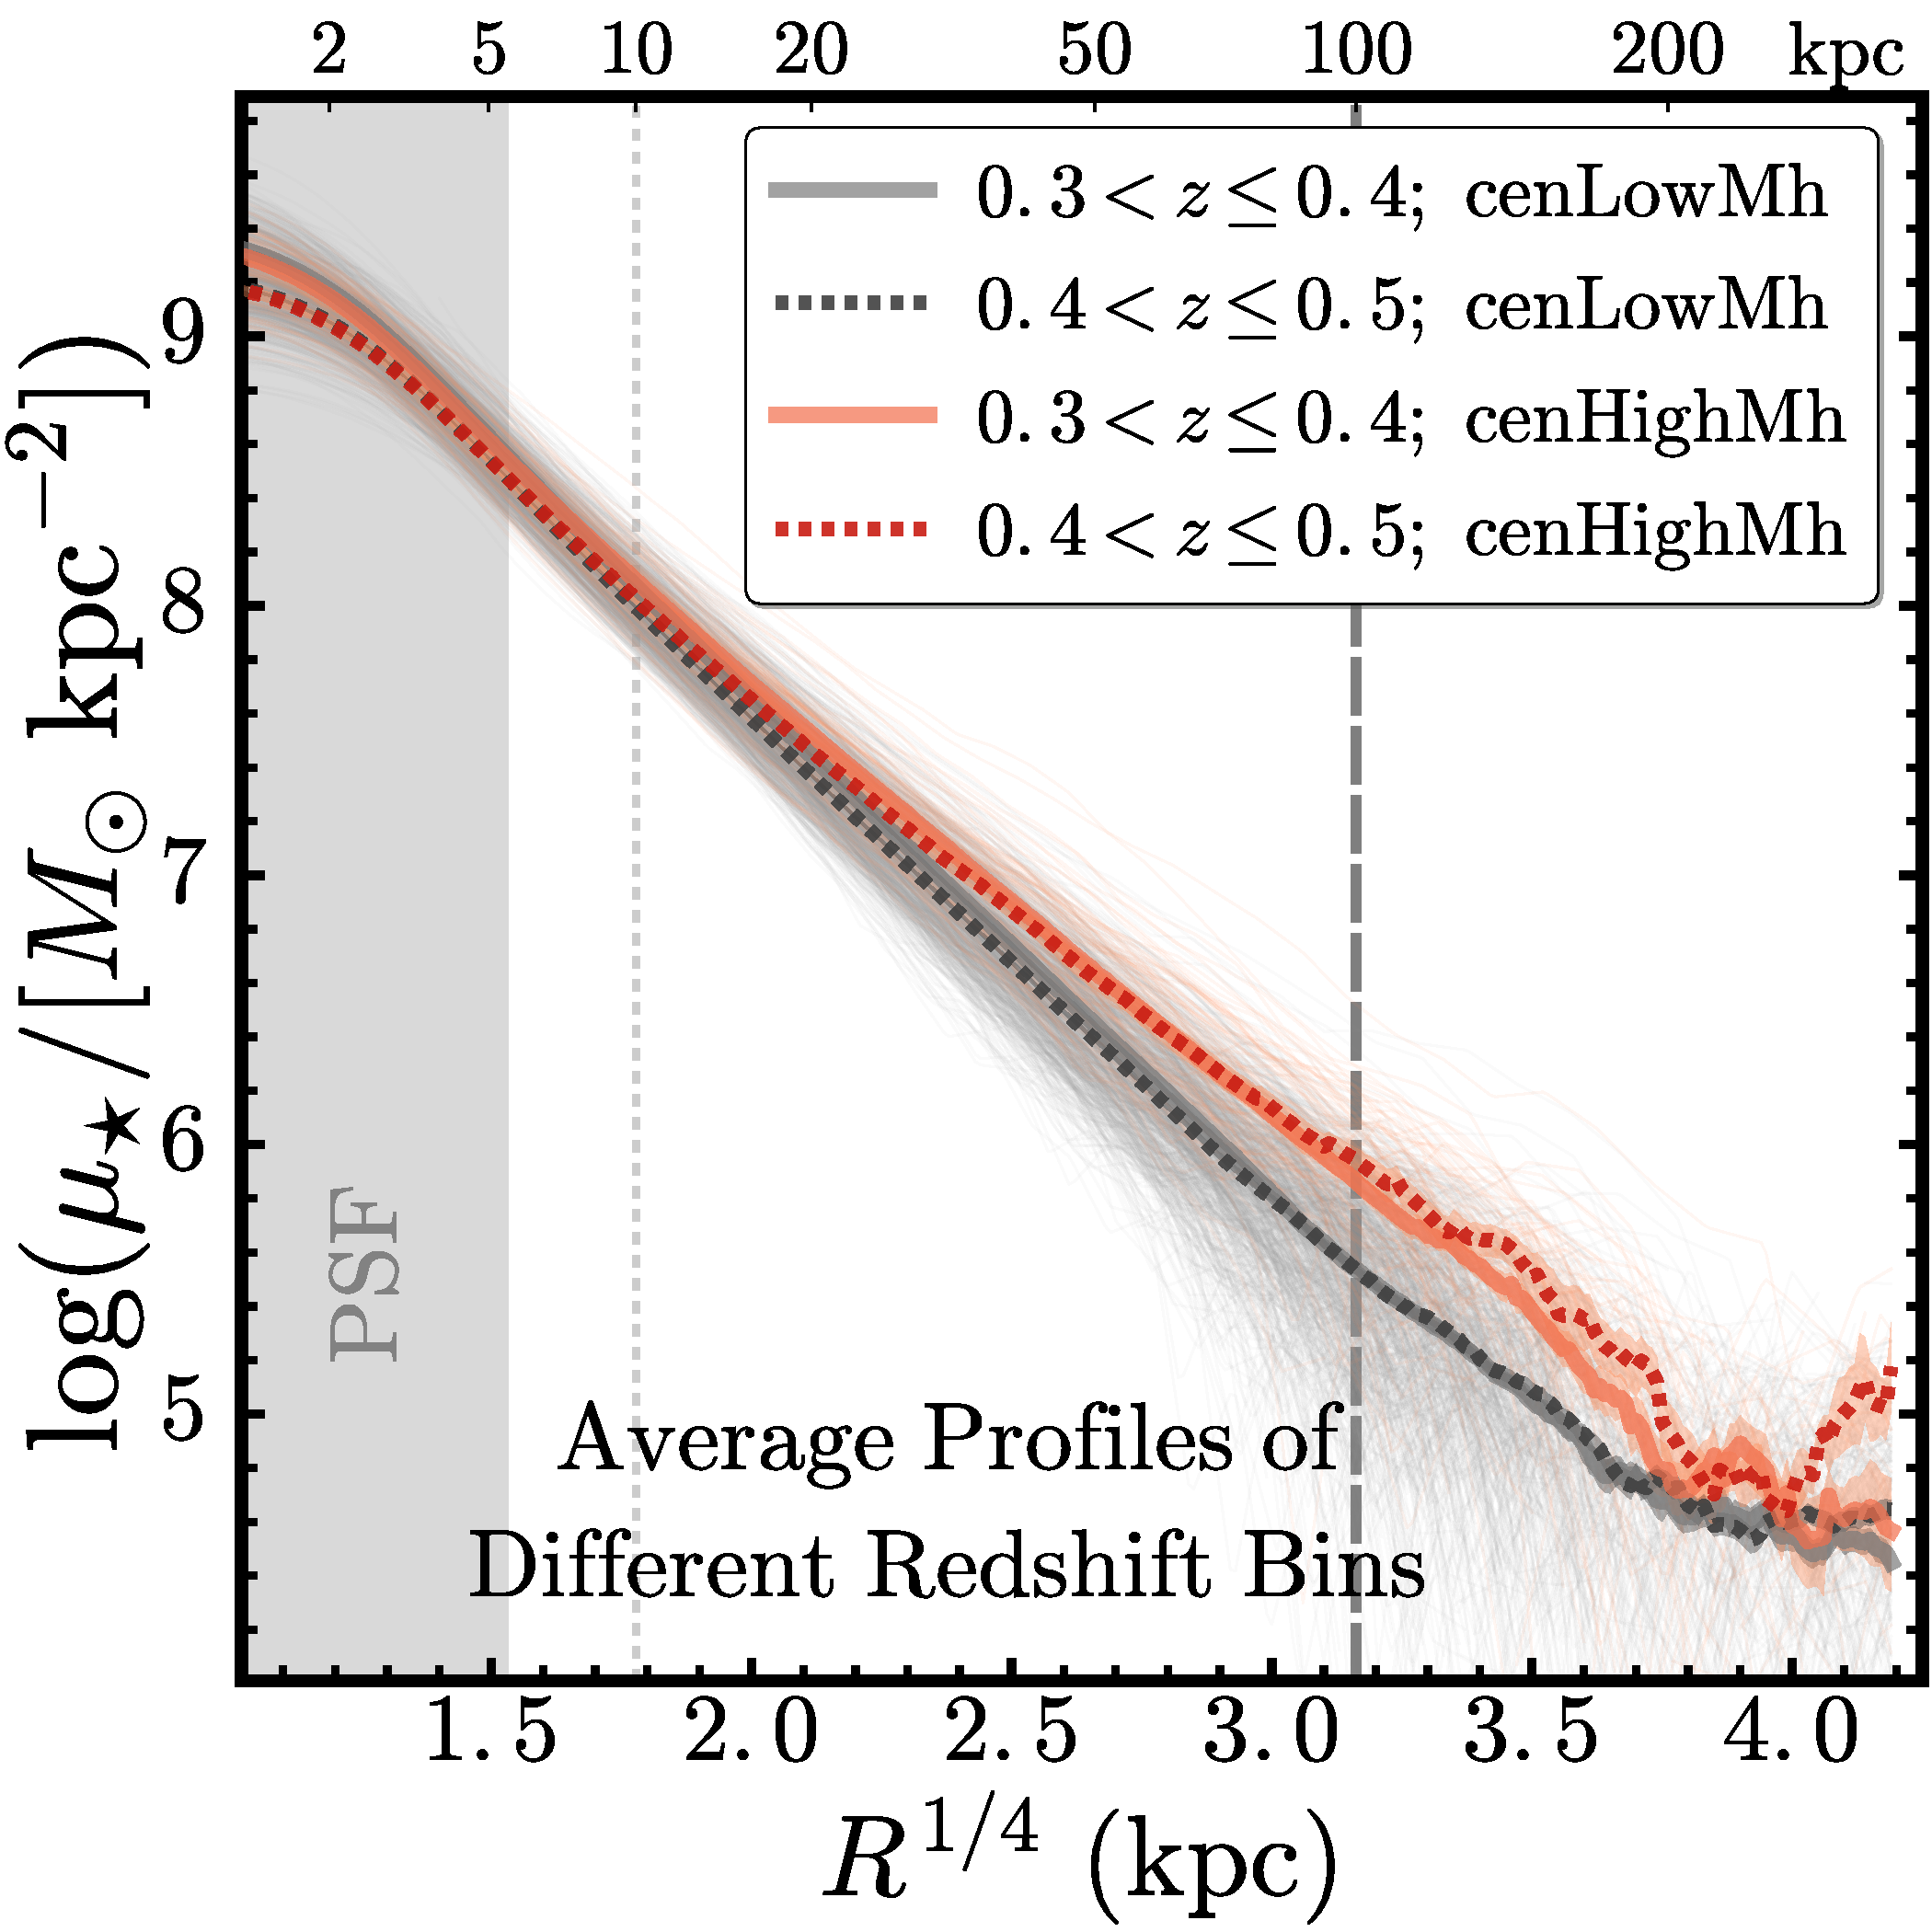
\includegraphics[width=8.2cm]{fig/redbcg_avg_prof_z}
    \caption{
        Comparison of \mden{} profiles of \rbcg{} (orange-red) and \nbcg{} 
        (grey-black) at $11.6 \le$\logmtot$< 11.9$ in redshift bins of 
        $0.3\leq z<0.4$ (solid lines) and $0.4\leq z<0.5$ (dash lines). 
        We show the individual profile in the background using much thinner line, 
        and highlight the median profiles using thicker line and darker color.
        }
    \label{fig:avg_prof_z}
\end{figure}    
%% ------------------------------------------------------------------------------------ %% 

    Given the redshift range for our samples, it is important to evaluate 
    the impacts from the physical extend of seeing and the imaging depth on the \mden{} 
    profiles at different redshift. 
    Under the same seeing, the \mden{} profile of galaxy at higher-$z$ is more 
    vulnerable to the PSF smearing effect at the center. 
    It is also harder to reach to the same \mden{} level under the same imaging depth 
    due to cosmological dimming and background noise. 
    
    In Fig~\ref{fig:avg_prof_z}, we group the \rbcg{} and \nbcg{} galaxies within 
    $11.6 \le$\logmtot$< 11.9$ into two $z$ bins ($0.3\leq z<0.4$ and $0.4\leq z<0.5$),
    and compare their \mden{} profiles. 
    In two redshift bins, the median \mden{} profiles from the same sample follow each 
    other very well outside 10 kpc, but become visibly different in the central 3-4 kpc,
    where the effect from seeing kicks in. 
    Meanwhile, the median \mden{} profiles of \rbcg{} and \nbcg{} in the same $z$ bin 
    are identical in the central region, which indicates similar average seeing 
    conditions.       
    This confirms that \mden{} profile at $> 5$ kpc is safe from the impacts of seeing 
    and difference in redshift.
    More importantly, it also suggests that, once the redshift distributions are 
    carefully matched, the difference of \mden{} profile is likely to be physical 
    even in the central region.  
%% ------------------------------------------------------------------------------------ %% 

%% ------------------------------------------------------------------------------------ %% 
\section{Match the \rbcg{} and \nbcg{} samples in \mstar{} and redshift distributions}
    \label{app:match}
    
%% ------------------------------------------------------------------------------------ %% 
\begin{figure*}
    \centering 
    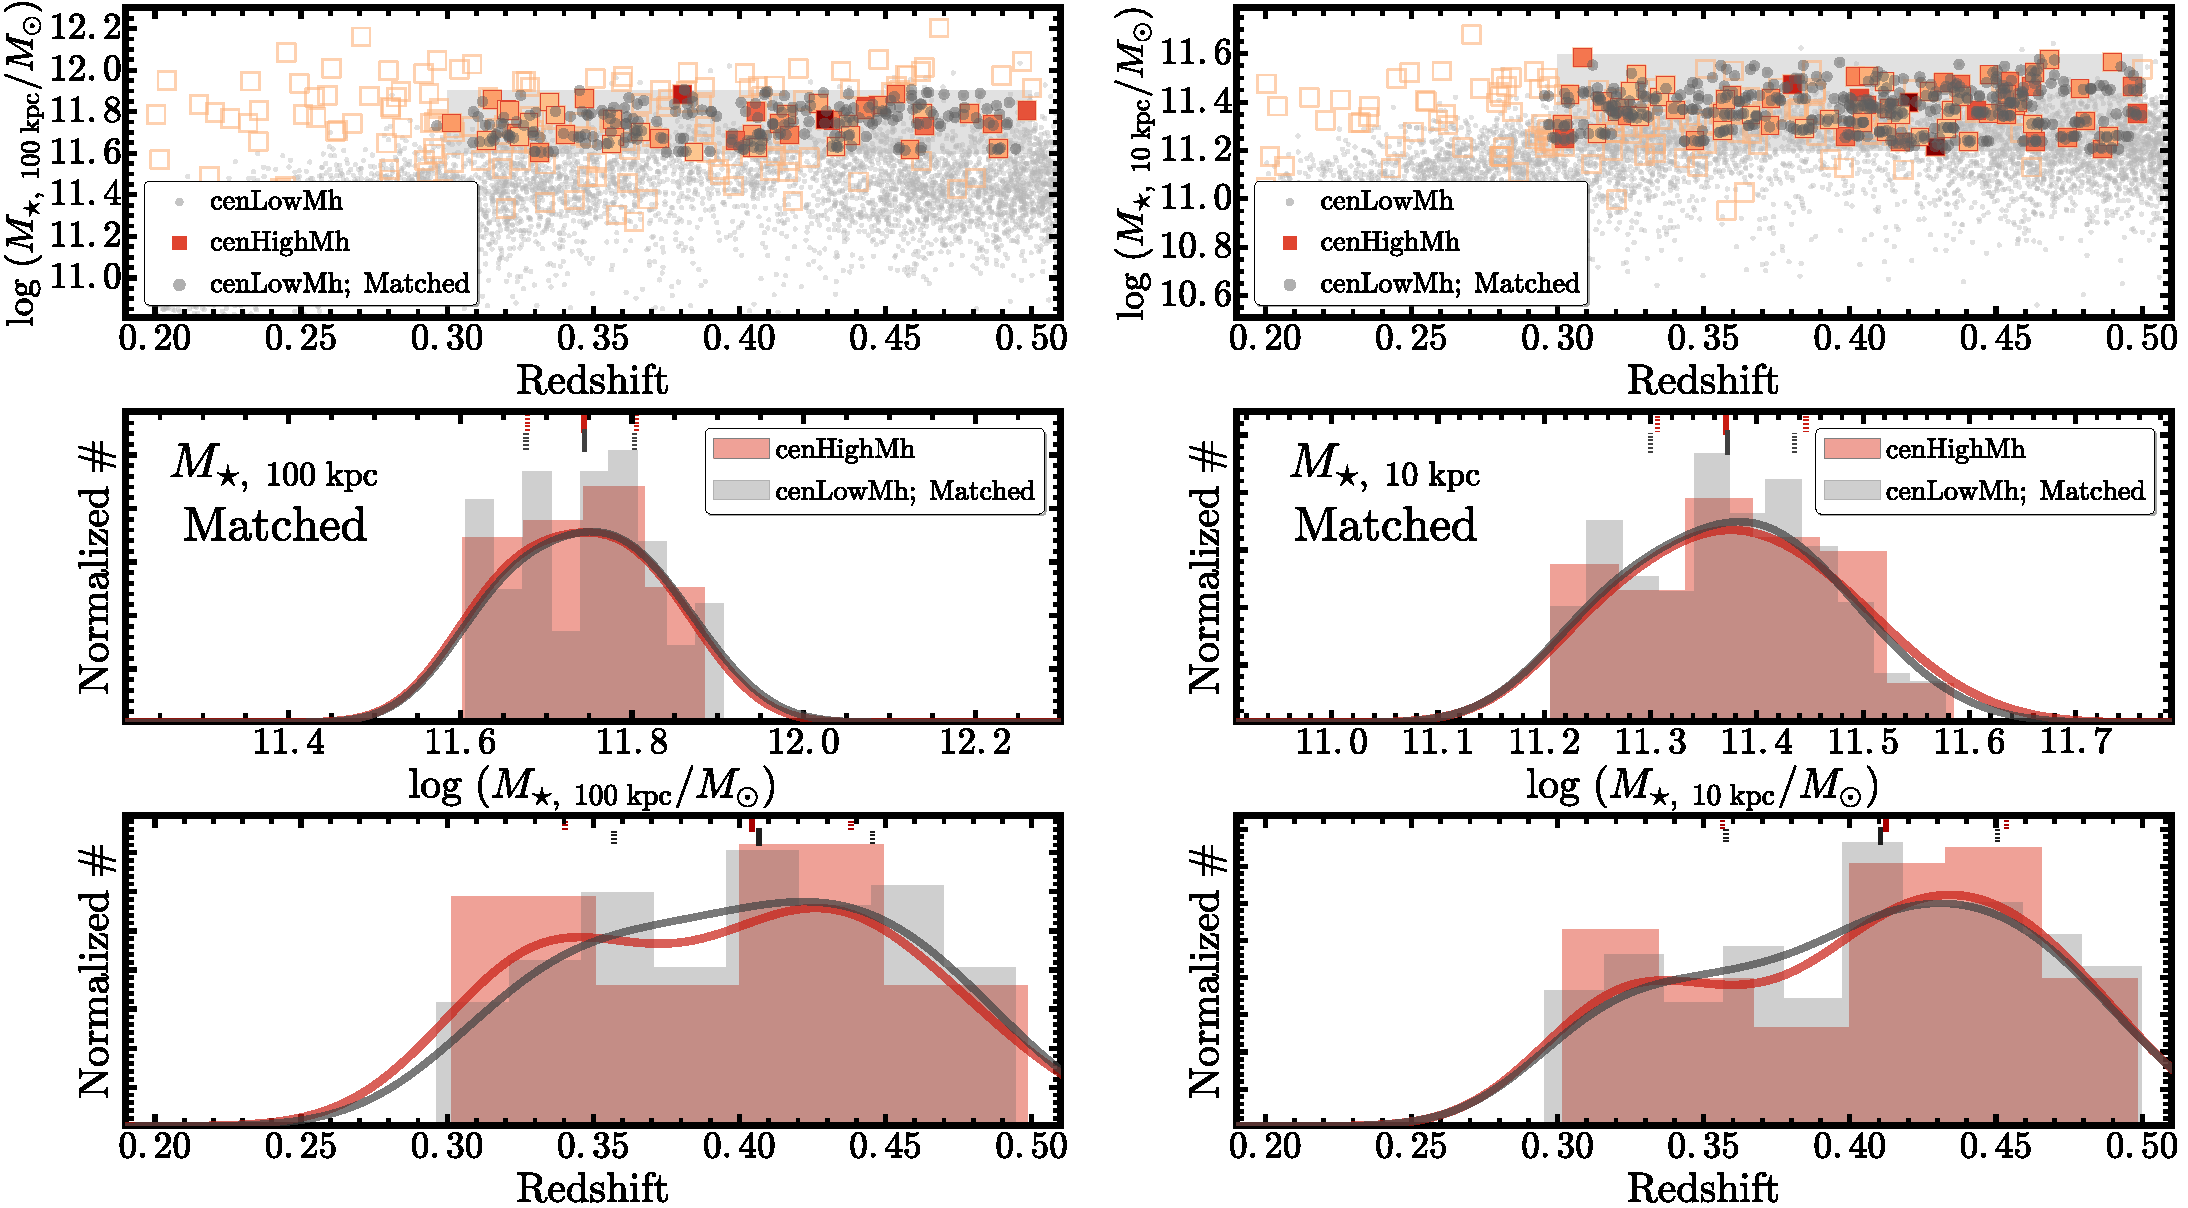
\includegraphics[width=15.0cm]{fig/redbcg_match}
    \caption{
        \textbf{Left figure} shows the details of the \mtot{}-matching process, 
        corresponding to the results shown in the left figure of   
        On the top panel, we show the overall distributions of \rbcg{} (light orange boxes) 
        and \nbcg{} (light grey dots) galaxies on the \mtot{}-$z$ plane.  
        And, we match the two sample in the \mtot{}-$z$ space outlined by the shaded region.
        We highlight the \rbcg{} galaxies in this region using bigger boxes in red frames, 
        whose size reflects the $P_{\mathrm{Cen}}$ value.  
        We also color-code them using the richness ($\lambda$) of the host cluster. 
        The matched \nbcg{} galaxies are highlighted using darker color and bigger dots. 
        To further evaluate the matching results, we show the distributions of \mtot{} 
        (middle panel) and redshift (bottom panel) separately. 
        On both panesl, we show the histograms along with their kernel density 
        distributions.  
        And, on the top of each panel, two sets of short vertical lines highlight the median 
        value (solid) and the inter-quartile (dash) of each distribution.~~~
        \textbf{Right figure} shows the similar matching results for the \minn{}-matched
        samples used for the right figure of Fig~\ref{fig:prof_1}.
        The format is exactly the same as the left one, except the \minn{} replaces the 
        \mtot{} in the top and middle panels.}
    \label{fig:match}
\end{figure*}
%% ------------------------------------------------------------------------------------ %% 

    As explained earlier, it is important to make sure the two samples have similar 
    distributions in both \mstar{} and redshift before comparing their median \mden{} 
    profiles.  
    Here we briefly describe the procedure used in this work. 
    Since the \rbcg{} sample is smaller in size, we always match the \nbcg{} sample to 
    it by searching for the $N$-nearest neighbours on the $M_{\star}$-redshift plane 
    using the KDTree algorithm in the \texttt{scikit-learn} Python library 
    (\citealt{scikit-learn}), and evaluate the quality of the match using the 
    distributions of both parameters (as shown in Fig~\ref{fig:match}). 
 
    As we only keep the unique \nbcg{} galaxies in the matched sample, we manually 
    adjust the value of $N$ to achieve the best match. 
    When the redshift distribution of the \rbcg{} sample becomes bi-model, we also try 
    to split the sample into two redshift bins and match them separately. 
    Typically $N$ is between 3 to 8.
    In Fig~\ref{fig:match}, we demonstrate this procedure using the results for 
    the \mtot{}-matched (Left) and the \minn{}-matched samples in Fig~\ref{fig:prof_1}
    (Right), and the two samples are well matched in the distributions of \mtot{}
    (or \minn{}) and redshift.  
    For all the comparisons of \mden{} profiles in this work, we match the samples 
    in the same way, and make sure the match has the same quality. 
%% ------------------------------------------------------------------------------------ %% 

    
%% ------------------------------------------------------------------------------------ %% 
\section{Robustness of the \mden{} Differences} 
	\label{app:robust}

%% ------------------------------------------------------------------------------------ %% 
  \begin{figure*}
      \centering 
      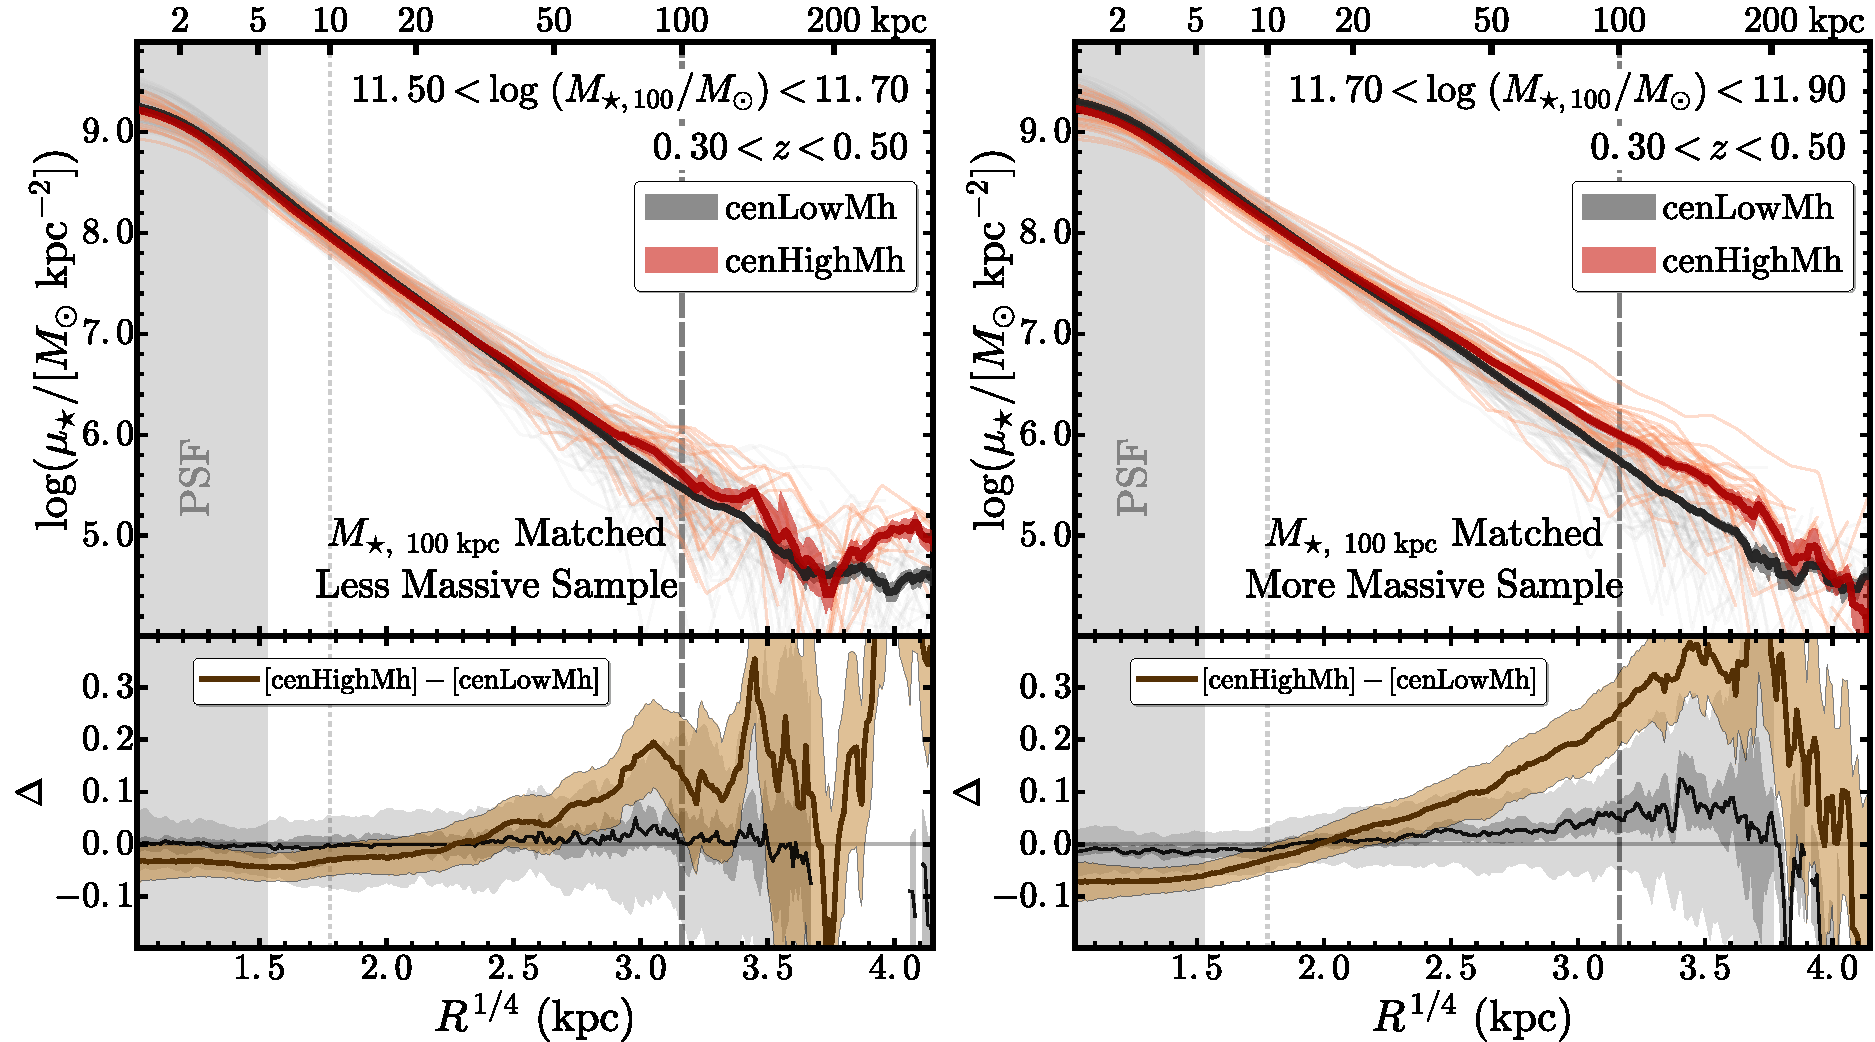
\includegraphics[width=15.5cm]{fig/redbcg_prof_2}
      \caption{
          Comparisons of the \mden{} profiles for \mtot{}-matched \rbcg{} 
          (orange-red) and \nbcg{} (grey-black) galaxies in lower (left; [11.5,11.70]) 
          and higher (right; [11.7, 11.9]) \mtot{} bins. 
          Other formats are in consistent with the right figure of Fig~\ref{fig:prof_1}.
          The difference in median profiles is more significant in higher \mtot{} bin.
          }
      \label{fig:prof_2}
  \end{figure*}
%% ------------------------------------------------------------------------------------ %% 

%% ------------------------------------------------------------------------------------ %% 
  \begin{figure*}
      \centering 
      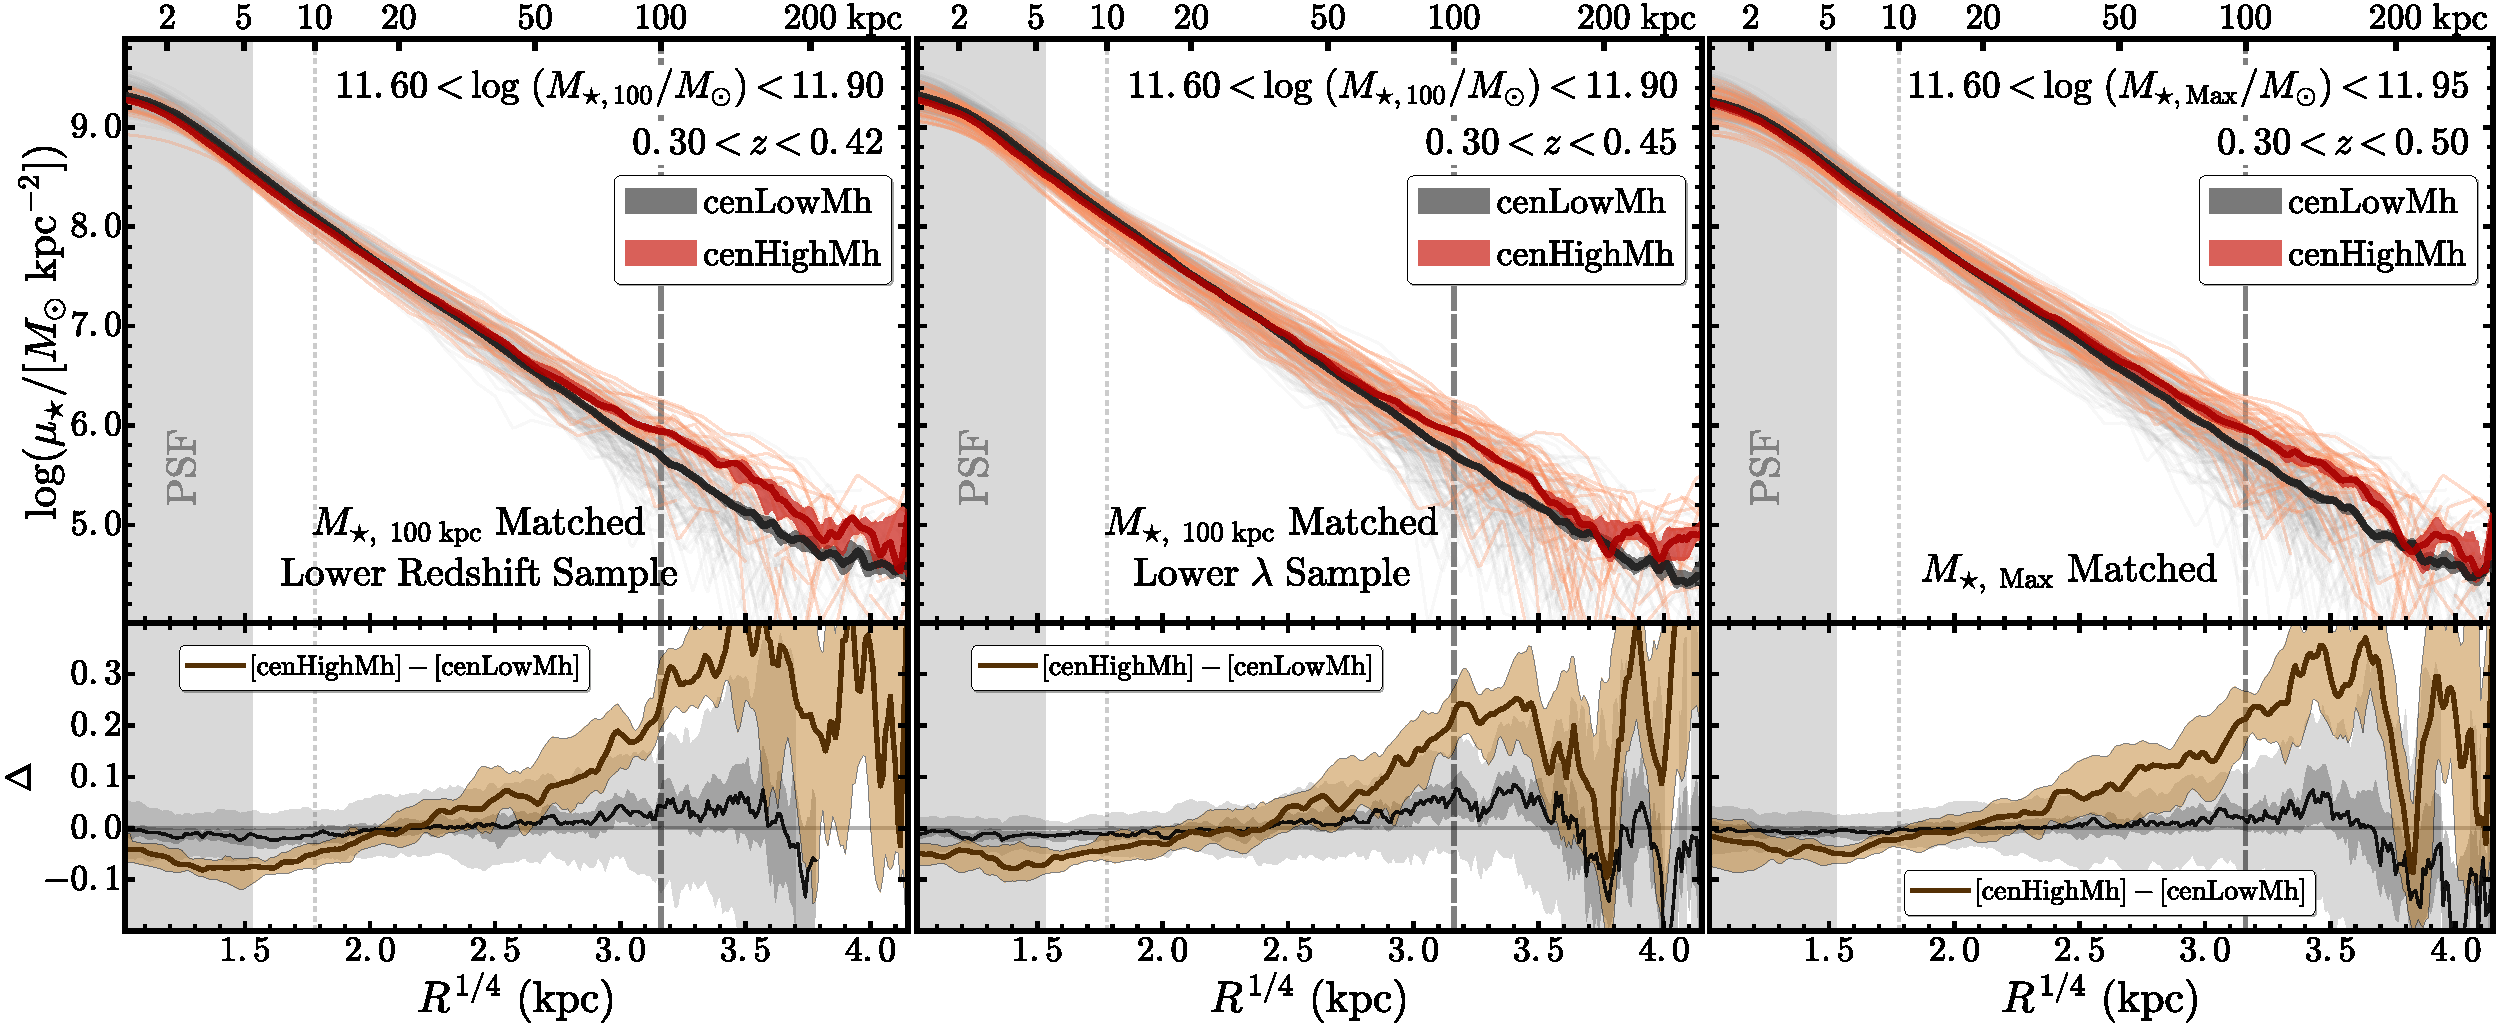
\includegraphics[width=\textwidth]{fig/redbcg_prof_3}
      \caption{
        Comparisons of the \mden{} profiles for \rbcg{} (orange-red) and \nbcg{} 
      	(grey-black) galaxies that are matched using proxies of total \mstar{}. 
        The formats are in consistent with the right figure of Fig~\ref{fig:prof_1}.
        The differences are, here, the samples are matched in slightly differnt ways. 
        From left to right: a) using samples at lower redshift ($0.3 < z < 0.4$); 
        b) using \rbcg{} sample with $\lambda > 20$ instead of 30; 
        c) using \mstar{} within 150 kpc instead of 100 kpc.
        The results are broadly consistent with the one in Fig~\ref{fig:prof_1}.
        }
      \label{fig:prof_3} 
  \end{figure*}
%% ------------------------------------------------------------------------------------ %% 

%% ------------------------------------------------------------------------------------ %% 
  \begin{figure*}
      \centering 
      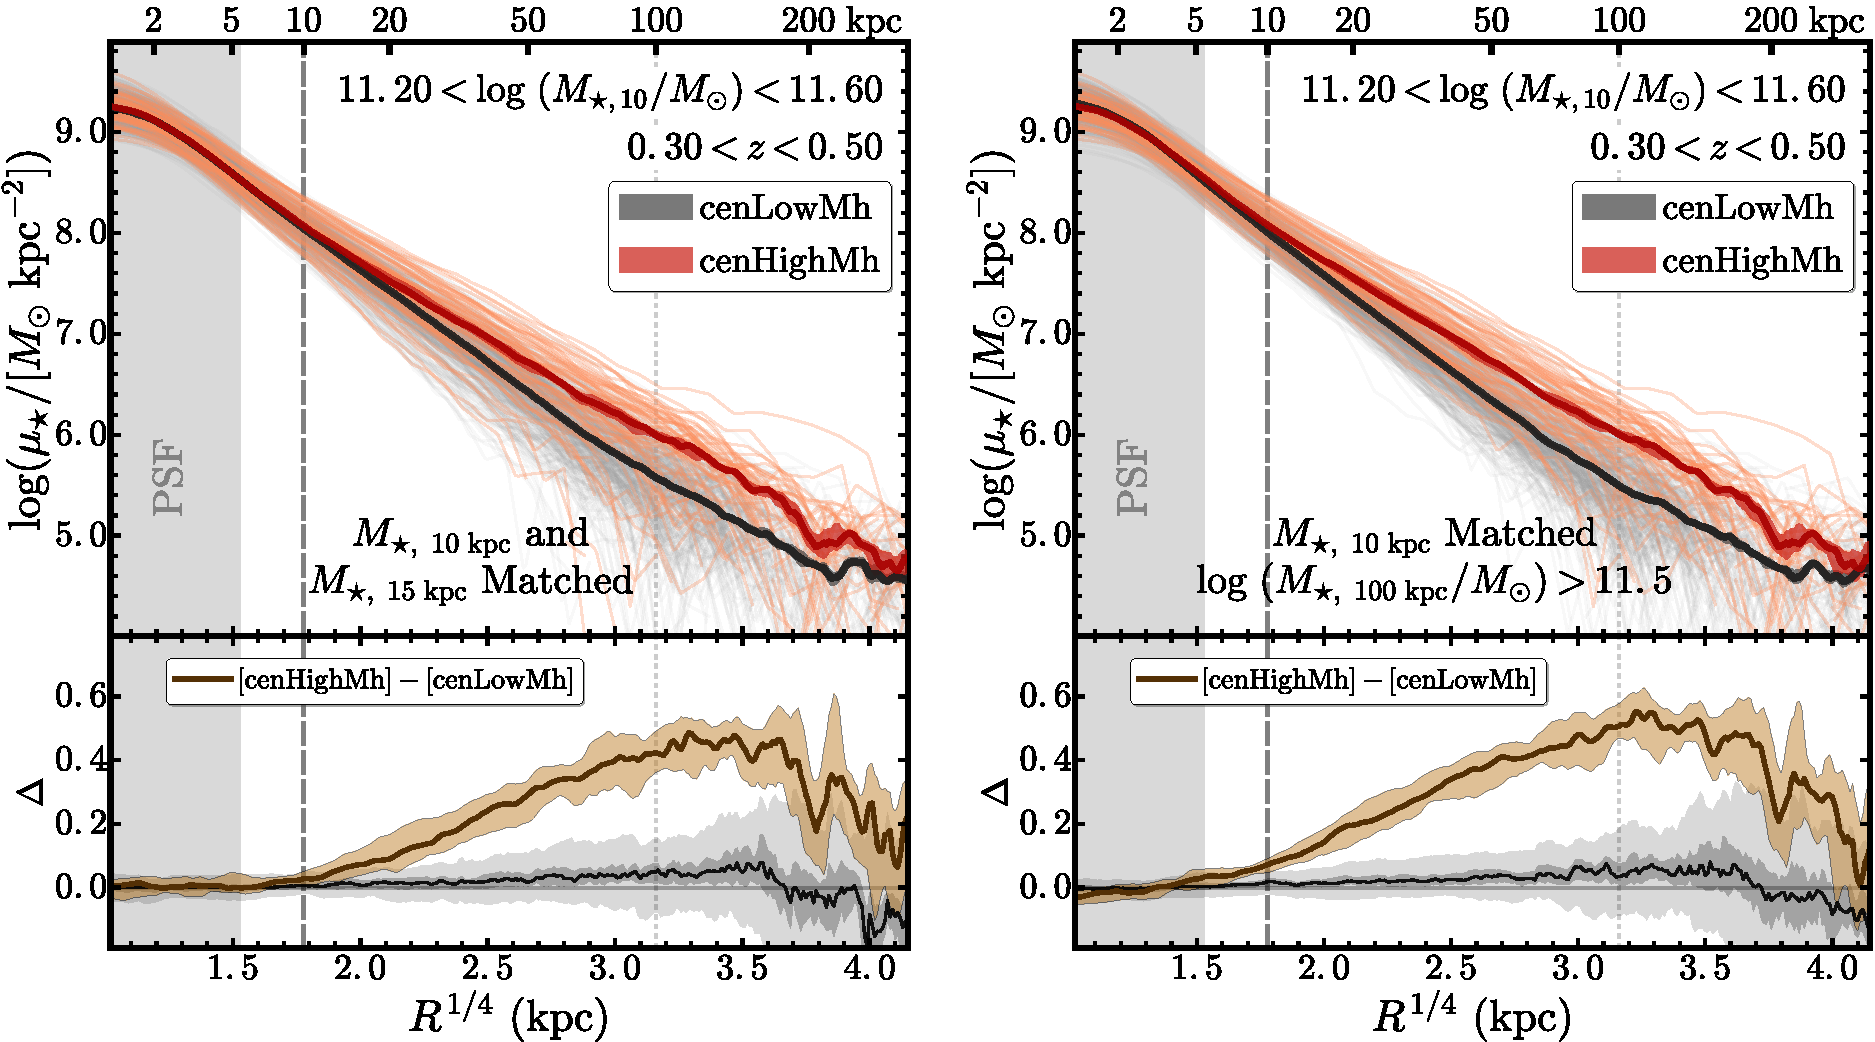
\includegraphics[width=15.5cm]{fig/redbcg_prof_4}
      \caption{
          Comparisons of the \mden{} profiles for \rbcg{} (orange-red) and \nbcg{} 
          (grey-black) galaxies that are matched using the \mstar{} enclosed in the 
          inner region. 
          Left panel shows the results after matching the \minn{} and \meff{} together, 
          and the right panel shows the results when only the \logmtot{}$\ge 11.5$
          \rbcg{} and \nbcg{} galaxies are included.
          Other formats are in consistent with the right figure of Fig~\ref{fig:prof_1}.
          }
      \label{fig:prof_4} 
  \end{figure*}
%% ------------------------------------------------------------------------------------ %% 

    In Fig~\ref{fig:prof_1}, we compare the \mden{} profiles of \mtot{}- and 
    \minn{}-matched samples of \rbcg{} and \nbcg{} galaxies, and here we test the 
    robustness of the results using a few extra tests that are illustrated in
    Fig~\ref{fig:prof_2}, Fig~\ref{fig:prof_3}, and Fig~\ref{fig:prof_4}, and 
    are briefly described here:   
    
    \begin{enumerate}
        
        \item In Fig~\ref{fig:prof_2}, we group the samples into two \mtot{} bins. 
            Given the small sample size, we extend slightly toward lower \mtot{} range 
            ($11.5 \leq \log (M_{\star,\ 10\mathrm{kpc}}/M_{\odot}) < 11.7$ and 
             $11.7 \leq \log (M_{\star,\ 10\mathrm{kpc}}/M_{\odot}) < 11.9$). 
            Although the smaller sample leads to larger statistical uncertainties, 
            we can still see similar structural differences in both \mtot{} bins, 
            and the difference becomes more significant in the higher \mtot{} bin.  
            For the lower \mtot{} bin, the difference in the inner region becomes 
            quite uncertain, while the difference in the outskirt is still visible. 
            This potentially suggests that the environmental dependence of structure 
            also varies with \mstar{}, an important implication deserves more 
            investigations in the future.   

        \item On the left panel of Fig~\ref{fig:prof_3}, we match the \rbcg{} and 
            \nbcg{} samples in a lower redshift bins ($0.30 < z < 0.42$).
            Despite the larger uncertainties due to smaller samples, we find the 
            results are the same.
            
        \item On the middle panel of Fig~\ref{fig:prof_3}, we includes \rbcg{} 
            galaxies in poorer clusters ($20 < \lambda < 30$), which should result 
            in overlapped \mhalo{} distributions with the \nbcg{} samples 
            considering the typical uncertainty of $\lambda$.
            This makes the difference in the inner region slightly less significant, 
            but the overall results are the same. 
             
        \item On the right panel of Fig~\ref{fig:prof_3}, in stead of using \mtot{}, 
            we use the \mmax{}--the maximum \mstar{} by integrating the \mden{} 
            profiles to the largest radius allowed.  
            The \mmax{} values are less reliable than \mtot{} due to the 
            uncertainty of background subtraction and contamination from nearby 
            bright objects, but they can serve as different estimates of the ``total''
            \mstar{} of these galaxies.
            As shown in Section~\ref{sec:discussion}, they on average increase
            the \mstar{} by a little bit and affect the \rbcg{} more.
            The differences in the \mden{} profiles still remain very similar.
      
    \end{enumerate}
    
    We also test the robustness of the \mtot{}-matched results using the samples with 
    only spectroscopic redshift, the samples in the three GAMA fields, and the \rbcg{} 
    samples without the ones in very massive haloes ($\lambda > 40$).  
    Limited by space, we do not show these results here, but they all verify the 
    robustness of the results. 
    
    For the results from the \minn{}-matched samples: 
    
    \begin{enumerate}
    
        \item
            We match the two samples using both \minn{} and the \mstar{} within 15 kpc 
            at the same time.  
            This makes the two median \mden{} profiles very similar inside 10-15 
            kpc, while the result in the outskirt remains the same (left panel of 
            Fig~\ref{fig:prof_4}).
            Use \mstar{} within 5 or 20 kpc leads to the same conclusion. 
          
        \item 
            To make sure the two samples are comparable in their overall assembly history,
            we also try to only include the very massive galaxies (\logmtot{}$>11.5$)
            in both samples. 
            This excludes the \nbcg{} galaxies that are much less massive and 
            more ``compact'' in structure. 
            Yet, the results regarding the structural differences remain the same. 
          
    \end{enumerate}
%% ------------------------------------------------------------------------------------ %% 

%% ------------------------------------------------------------------------------------ %% 
\section{Stellar Mass Curve-of-Growth for Massive Central Galaxies} 
	\label{app:cog}
	
	In \S \ref{ssec:sbp_mtot} and Figure \ref{fig:prof_1}, we show the comparisons 
	of \mden{} profiles for massive central galaxies from the \rbcg{} and \nbcg{} 
	samples. 
	Although the differences in their median \mden{} profiles we revealed are robust 
	and systematic, they appear to be very subtle, especially in the inner region. 
	This is partly due to the logarithmic scale on the Y--axis for \mden{} profiles. 
	
	In Figure \ref{fig:cog}, we compare the same two samples after converting the 
	\mden{} profiles into: 
	
	\begin{enumerate}
	
	    \item ``Curve--of--growth'' of stellar mass--the cumulative \logms{} profiles
	        (upper panel).
	    
	    \item Fraction of \mtot{} within different radius (lower panel).
	
	\end{enumerate}
	
	These comparisons demonstrate the same results from different angles and 
	the systematic differences become more clear using the fraction of \mtot{}
	within different radius.  
	The comparison of cumulative \logms{} profiles also demonstrates that the 
	\rbcg{} and \nbcg{} samples have very similar median \mtot{}.  
    They help confirm that the distributions of stellar mass within 100 kpc indeed 
    have systematic differences between the massive central galaxies living in more 
    and less massive dark matter haloes. 

%% ------------------------------------------------------------------------------------ %% 

%% ------------------------------------------------------------------------------------ %% 
\begin{figure*}
    \centering
    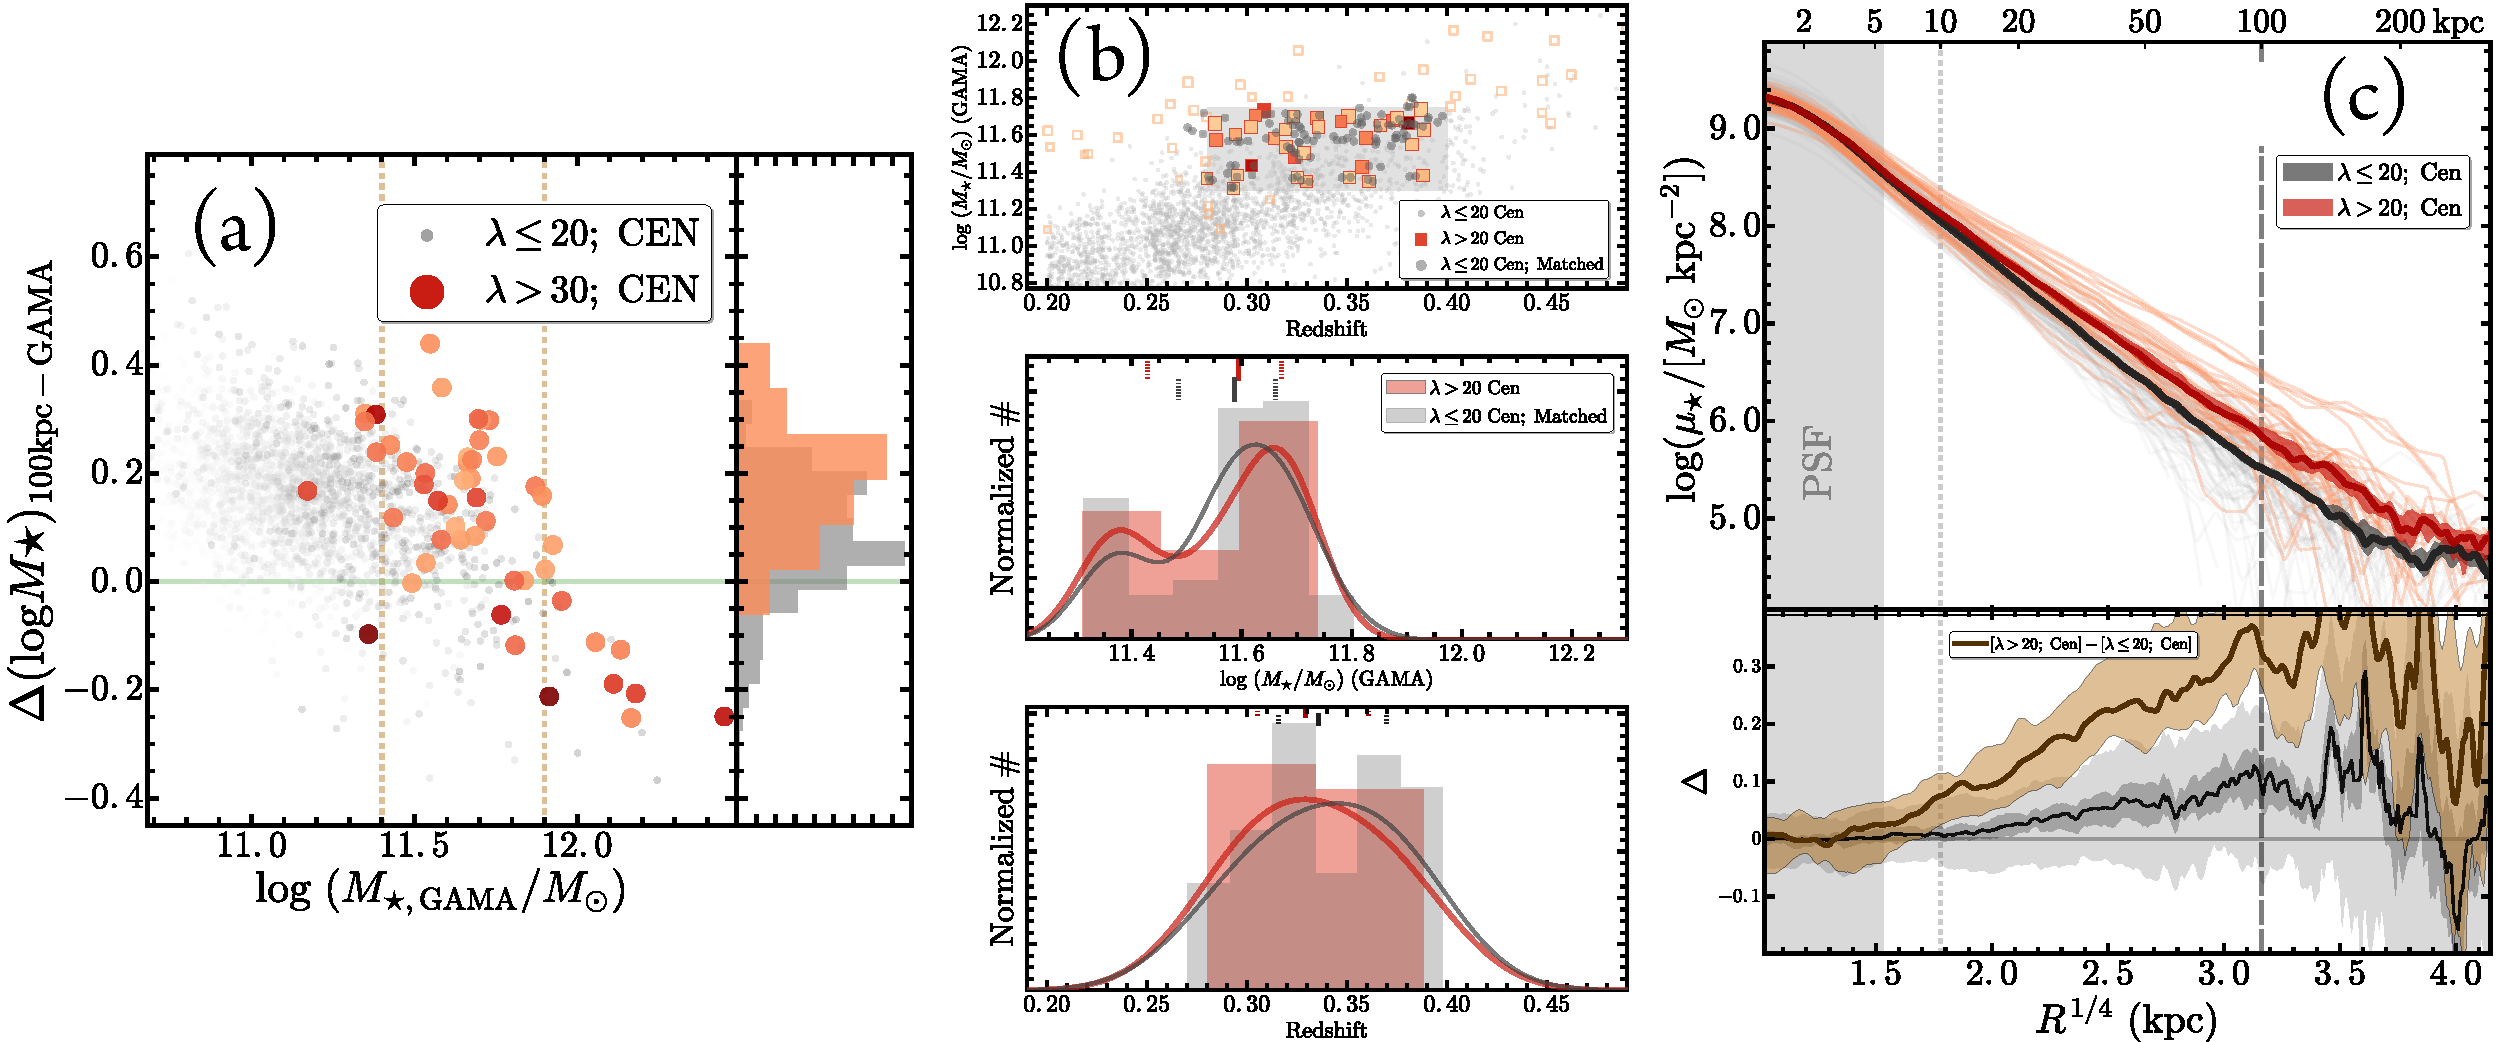
\includegraphics[width=16cm]{fig/redbcg_prof_gama_new}
    \caption{
        \textbf{Left:} comparison of \mstar{} estimated by the GAMA survey and 
        the \mtot{} using HSC images in this work. 
        We plot the \logmgama{} against the difference between \logmtot{} and \logmgama{}. 
        The two vertical lines highlight the mass range $11.4 \leq$\logmgama{}$<11.8$ 
        that is used for the comparison.~~
        \textbf{Right:} we compare the \mden{} profiles of \rbcg{} (orange-red) and 
        \nbcg{} (grey-black) galaxies using the samples matched on the 
        \mgama{}-$z$ plane at $11.4 \leq$\logmgama{}$<11.9$ and $0.28 \leq z < 0.4$. 
        The format is very similar to the ones in Fig~\ref{fig:prof_1}.}
    \label{fig:gama}
\end{figure*}
%% ------------------------------------------------------------------------------------ %% 


%% ------------------------------------------------------------------------------------ %% 
\section{Comparison of \mden{} profiles using \mstar{} from the GAMA survey}
    \label{app:gama} 

%% ------------------------------------------------------------------------------------ %% 
\begin{figure}
    \centering
    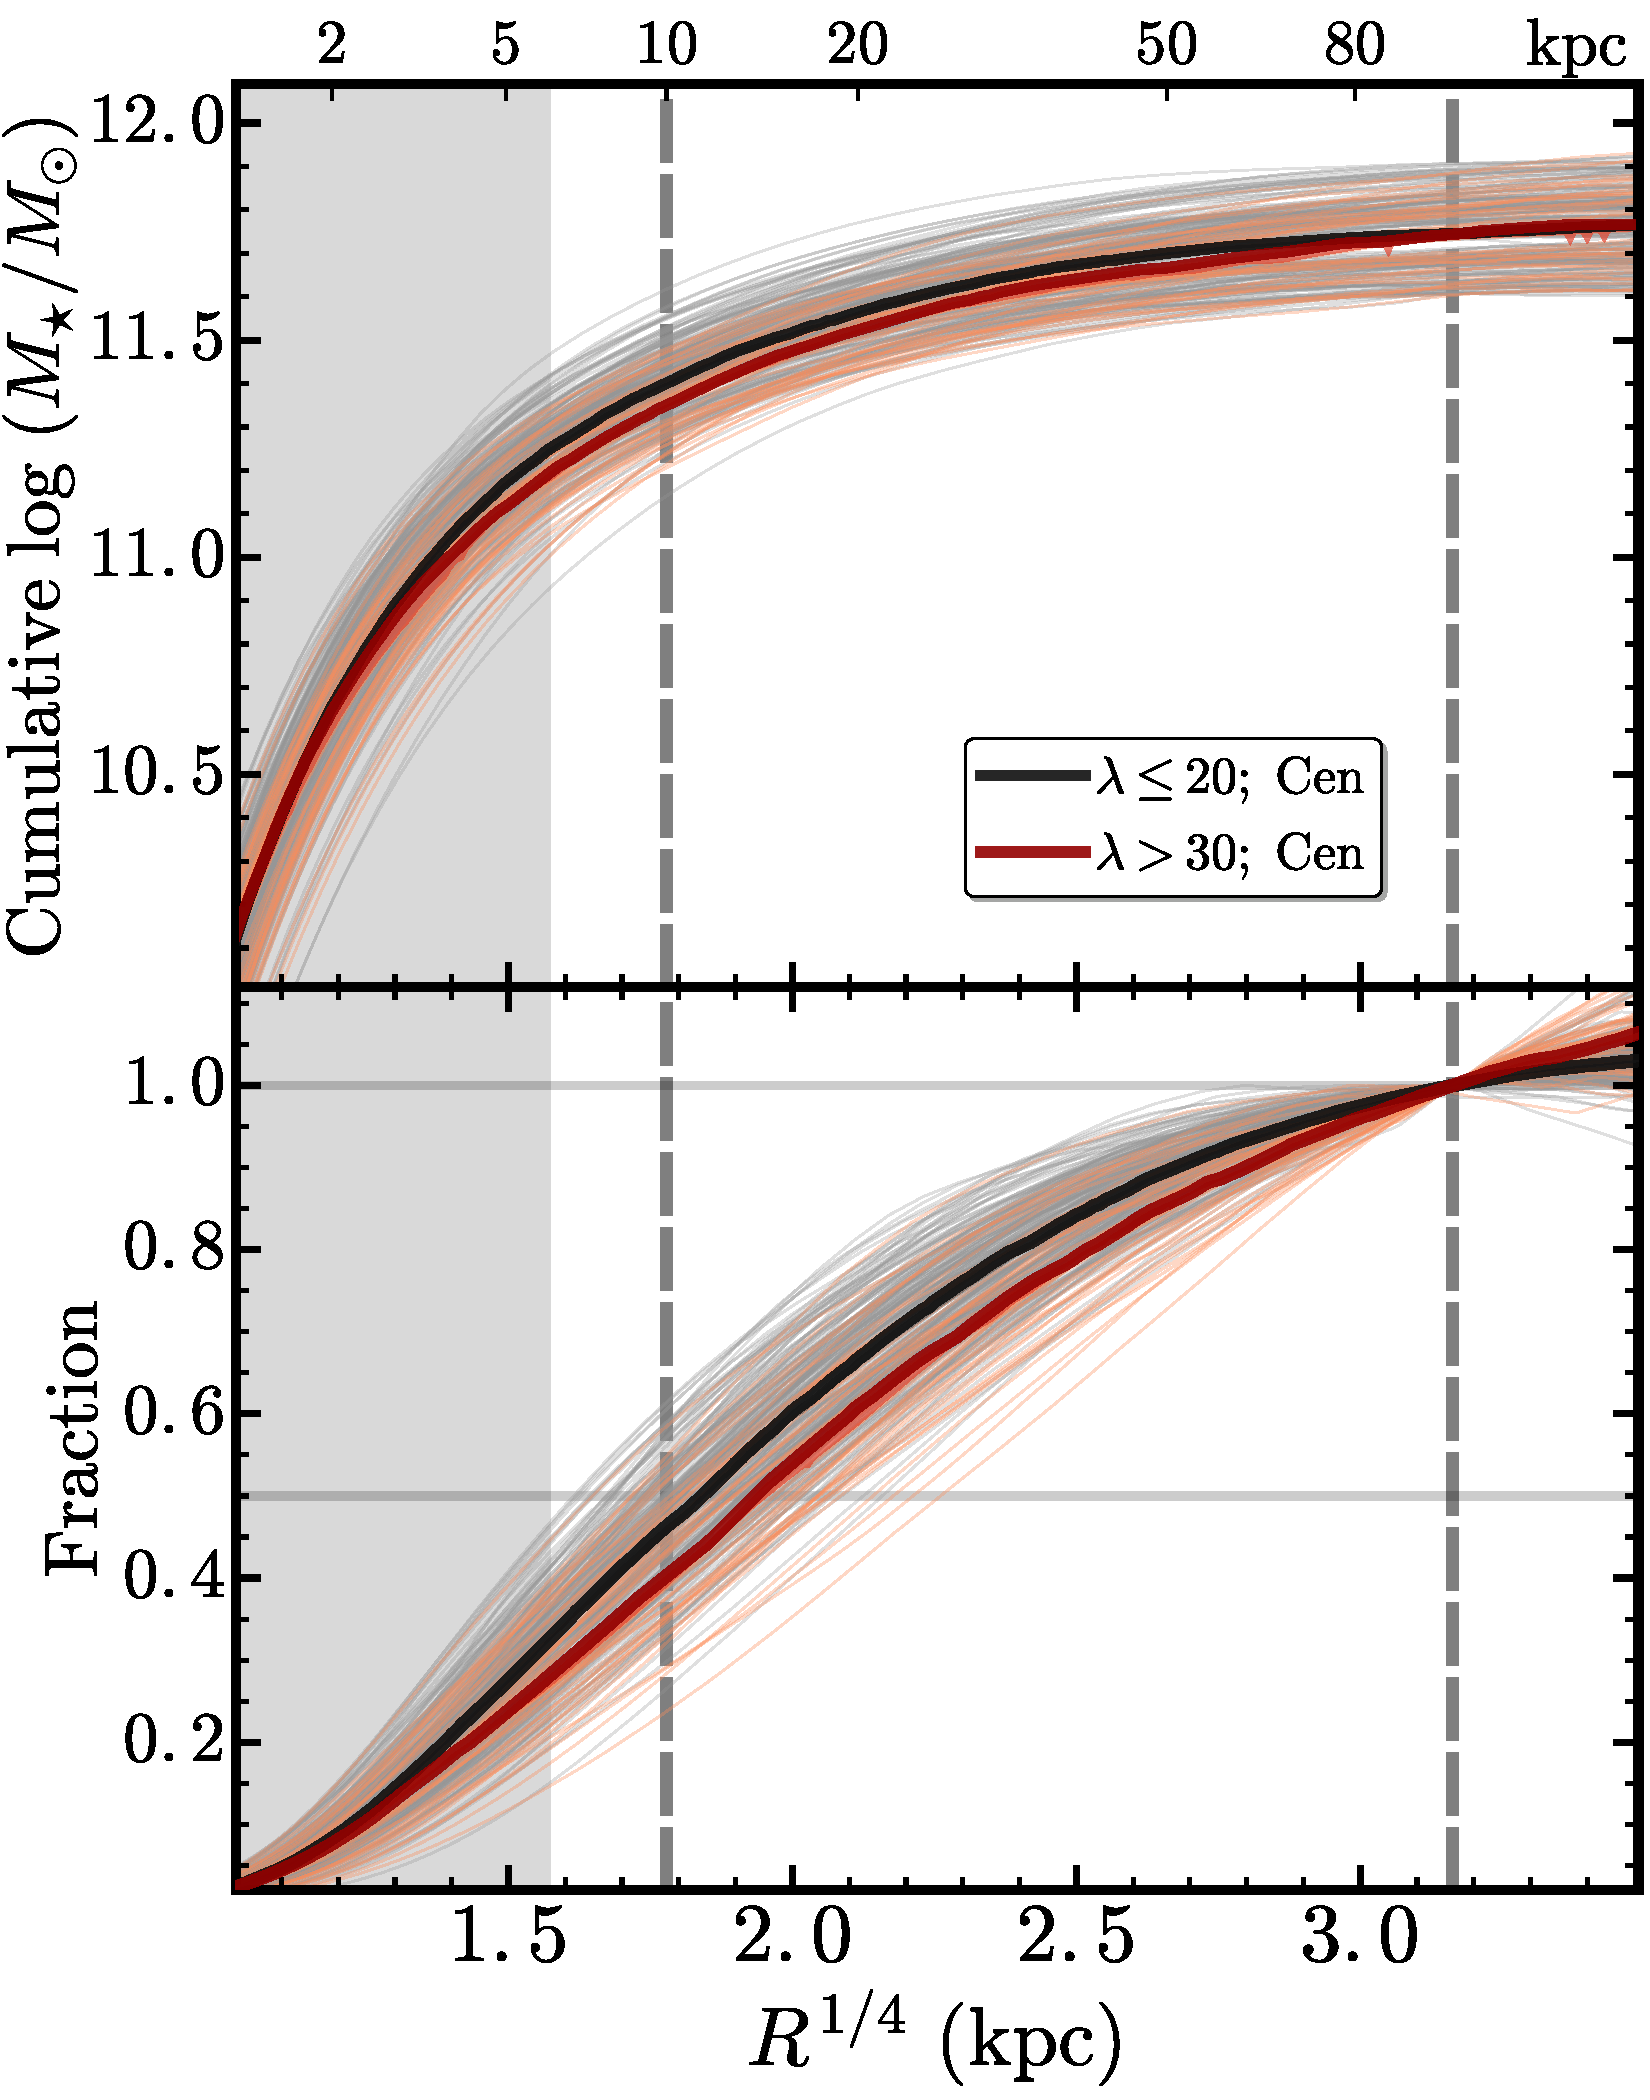
\includegraphics[width=\columnwidth]{fig/redbcg_prof_m100D}
    \caption{
        \textbf{Top:} comparison of the cumulative \mstar{} profiles for 
        \rbcg{} (orange--red) and \nbcg{} (grey--black) galaxies at fixed \mtot{}.~~
        \textbf{Bottom:} comparison of the fraction of \mtot{} within different radius 
        for the same samples at fixed \mtot{}. 
        Thicker and darker solid lines highlight the median profiles. 
        Other formats of the figure are similar to Figure \ref{fig:prof_1}. 
        Besides the region affected by seeing, the 10 and 100 kpc radius, we 
        also highlight the 50\% and 100\% values using horizontal grey lines on the 
        bottom panel. 
        }
    \label{fig:cog}
\end{figure}
%% ------------------------------------------------------------------------------------ %% 
    
    The GAMA survey greatly overlaps with the HSC survey, and it provides carefully 
    measured \mstar{} for large sample of galaxies (\citealt{Taylor2011}) that help 
    produce many interesting results (e.g. \citealt{Bauer2013, Ferreras2017}).
    They use 2-D single-\ser{} model to correct the total luminosity of the galaxy 
    (\citealt{Kelvin2012}), and derive the \m2l{} through optical-SED fitting 
    (BC03 model; Chabrier IMF) based on the PSF-matched aperture photometry. 
    Since the \ser{} model is generally more flexible than the \texttt{cModel} one, 
    it is therefore interesting to compare with the \rbcg{} and \nbcg{} galaxies 
    that also have spec-$z$ (at $z < 0.40$) and \mstar{} in GAMA DR2 
    (\citealt{Liske2015}) and see the impact of deep photometry again. 
    
    We summarize the results in Fig~\ref{fig:gama}.  
    On the left panel, we compare the differences between \mtot{} and \mgama{}. 
    HSC survey on average recovers more \mstar{} at high-\mstar{} end, which is 
    consistent with the expectation from deeper photometry, although the 
    systematic differences in the estimates of \m2l{} could play a role here. 
    Meanwhile, it is interesting see that, above \logmtot{}$> 11.8$, \mgama{} 
    becomes increasingly larger than \mtot{}, and most of these massive 
    galaxies have very high \ser{} index from the 2-D fitting. 
    This suggests that the single-\ser{} model is no longer an appropriate one to 
    describe very massive galaxies as it tends to over-estimate the \mstar{} the 
    inner and/or outer regions. 
    
    To verify the cause of the difference in \mstar{}, we further select samples 
    of \rbcg{} and \nbcg{} galaxies with matched \mgama{} and redshift 
    distributions (at $11.4 <$\logmgama{}$<11.8$; see Appendix \ref{app:match}), 
    and compare their \mden{} profiles (right panel). 
    Although these two subsamples are equally massive according to results from 
    GAMA survey, it is clear that the \rbcg{} galaxy has much more extended 
    outer envelope, even though its median \mden{} profile is very similar 
    to the \nbcg{} sample at $< 10$ kpc. 
    We can reproduce very the same trend with the luminosity density profiles 
    (with or without $k$-correction), suggesting that the inaccurate \ser{} 
    model definitely leads to under-estimate of \mstar{}.  
 
%% ------------------------------------------------------------------------------------ %% 


%% ------------------------------------------------------------------------------------ %%  
\bsp
\label{lastpage}
\end{document}
%% ------------------------------------------------------------------------------------ %% 
%%%%%%%%%%%%: End of the File %%%%%%%%%%%%
%% ------------------------------------------------------------------------------------ %% 